\documentclass[11pt]{article} % Font size
\usepackage{amsmath, amsfonts, amsthm,url} % Math packages
\usepackage{changepage}

\newenvironment{subs}
  {\begin{adjustwidth}{3em}{0pt}}
  {\end {adjustwidth}}
\usepackage{imakeidx} % index

\usepackage{listings} % Code listings, with syntax highlighting

\usepackage[english]{babel} % English language hyphenation

\usepackage{graphicx} % Required for inserting images
\graphicspath{{Figures/}{./}} % Specifies where to look for included images (trailing slash required)

\usepackage{booktabs} % Required for better horizontal rules in tables

\numberwithin{equation}{section} % Number equations within sections (i.e. 1.1, 1.2, 2.1, 2.2 instead of 1, 2, 3, 4)
\numberwithin{figure}{section} % Number figures within sections (i.e. 1.1, 1.2, 2.1, 2.2 instead of 1, 2, 3, 4)
\numberwithin{table}{section} % Number tables within sections (i.e. 1.1, 1.2, 2.1, 2.2 instead of 1, 2, 3, 4)

\setlength\parindent{0pt} % Removes all indentation from paragraphs

\usepackage{enumitem} % Required for list customisation
% \setlist{noitemsep} % No spacing between list items

%----------------------------------------------------------------------------------------
%	DOCUMENT MARGINS
%----------------------------------------------------------------------------------------

\usepackage{geometry}
	\geometry{
		a4paper,
		total={160mm,245mm},
		left=1in,
		right=1in,
	}

\usepackage{lipsum}
\usepackage{layout}


%	FONTS

\usepackage[utf8]{inputenc} % Required for inputting international characters
\usepackage[T1]{fontenc} % Use 8-bit encoding

\usepackage{fourier} % Use the Adobe Utopia font for the document

%----------------------------------------------------------------------------------------
%	SECTION TITLES
%----------------------------------------------------------------------------------------

\usepackage{sectsty} % Allows customising section commands

\sectionfont{\vspace{6pt}\normalfont\bfseries\boldmath} % \section{} styling
\subsectionfont{\normalfont\bfseries} % \subsection{} styling
\subsubsectionfont{\normalfont\bfseries} % \subsubsection{} styling
\paragraphfont{\normalfont\scshape} % \paragraph{} styling

%----------------------------------------------------------------------------------------
%	HEADERS AND FOOTERS
%----------------------------------------------------------------------------------------

\usepackage{scrlayer-scrpage} % Required for customising headers and footers

\ohead*{} % Right header
\ihead*{} % Left header
\chead*{} % Centre header

\ofoot*{} % Right footer
\ifoot*{} % Left footer
\cfoot*{\pagemark} % Centre footer

\usepackage[normalem]{ulem}
\useunder{\uline}{\ul}{}

 % Include 
\title{	
	\date{}
	\normalfont\Large
	\textsc{Software Engineering (Sessional) Final Report }\\ % Your university, school and/or department name(s)
	\textsc\centering{ Course: CSE-434 }\\ % Your university, school and/or department name(s)
	
    \begin{figure}[h] % [h] forces the figure to be output where it is defined in the code (it suppresses floating)
        \centering
        
\includegraphics[width=0.3\columnwidth]{CUET_Vector_logo} % Example image
        %\caption{European swallow.}
    \end{figure}
    
	 % Your university, school and/or department name(s)
	\vspace{25pt} % Whitespace
	\rule{\linewidth}{2pt}\\ % Thin top horizontal rule
	\vspace{20pt} % Whitespace
	{\huge Automobile Maintenance and Breakdown Assistance}\\ % The assignment title
	\rule{\linewidth}{2pt}\\ % Thin top horizontal rule
	\vspace{110pt} % Whitespace
	\centering	
	% Please add the following required packages to your document preamble:
% \usepackage[normalem]{ulem}
% \useunder{\uline}{\ul}{}
	\centering
	\begin{tabular}{l|l}
	\multicolumn{1}{c|}{Name} & \multicolumn{1}{c}{ID} \\ \hline
	Faria Zarin Subah        & 1504027                \\ \hline
	Adrita Barua       & 1504015               \\ \hline
	Tarek Hossain          & 1504014               
	\end{tabular}
	
	\vspace{105pt} % Whitespace
	\normalfont\Large
	\textsc{Department of Computer Science \& Engineering}\\
	
	\normalfont\Large
	\textsc{Chittagong University of Engineering \& Technology}\\
}
 % title
\usepackage{tabularx}
\usepackage{multirow}
\usepackage{amsmath}
% \author{} % Your name

\date{} % Today's date (\today) or a custom date

\makeindex
  
\begin{document}
\maketitle % Print the title

\begin{center}
 
	\Large\textbf{Team Members}
\end{center}
\begin{table}[ht]
\centering
\begin{tabular}{|c|c|c|c|c|c|c|}
\hline
Photo 
& Name                    
& ID
& Email 
& Contact No. 
& \begin{tabular}[c]{@{}c@{}}Total\\ Credit \\ Passed\end{tabular}
& \begin{tabular}[c]{@{}c@{}}CGPA  \\ acquired\end{tabular}
\\ \hline
	
\begin{tabular}[c]{@{}c@{}}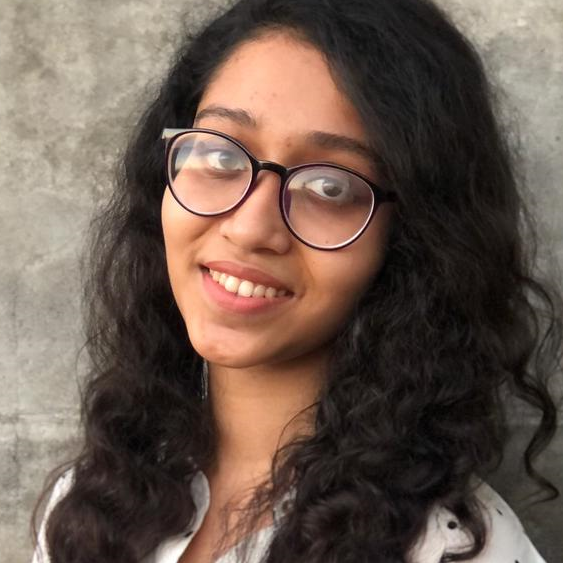
\includegraphics[scale=.11]{1504027 img.png} \end{tabular}
& \begin{tabular}[c]{@{}c@{}}Faria Zarin Subah\end{tabular} 
& 1504027 
& \begin{tabular}[c]{@{}c@{}}u1504027@\\student.cuet.ac.bd\end{tabular} 
& 01791150598 
& 138 
& 3.81
\\ \hline

\begin{tabular}[c]{@{}c@{}}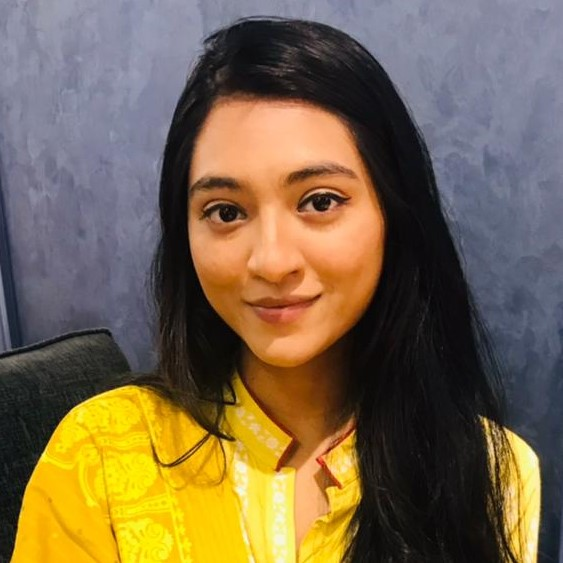
\includegraphics[scale=.11]{im2.jpg}\end{tabular} 
& \begin{tabular}[c]{@{}c@{}}Adrita Barua \end{tabular} 
& 1504015 & \begin{tabular}[c]{@{}c@{}}u1504015@\\student.cuet.ac.bd\end{tabular}
& 01862881704
& 138  
& 3.64
\\ \hline
	\begin{tabular}[c]{@{}c@{}}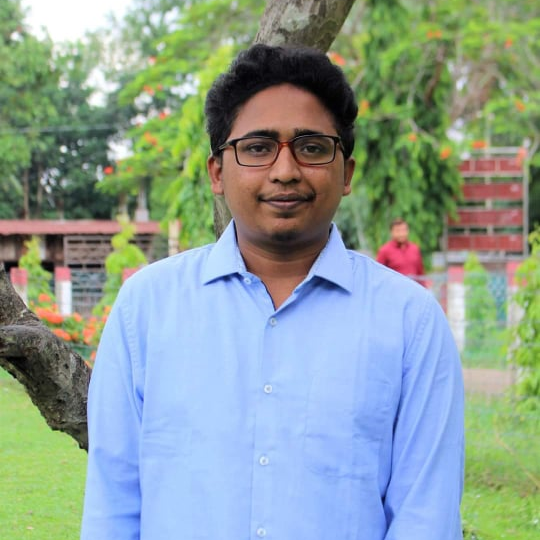
\includegraphics[scale=.11]{tarek.png}\end{tabular}
	& \begin{tabular}[c]{@{}c@{}}Tarek Hossain  \end{tabular}  
	& 1504014 
	& \begin{tabular}[c]{@{}c@{}}u1504014@\\student.cuet.ac.bd\end{tabular}
	& 01859601184
	& 132 
	& 3.01
\\ \hline
\end{tabular}
\end{table}
\newpage
\tableofcontents
\pagebreak
\listoffigures

\listoftables
\pagebreak

\section{Introduction}
In our Software Engineering (Sessional) course, CSE-434, it is required to develop a software project following prescribed software engineering principles and framework. Our project entitled Automobile Maintenance and Breakdown Assistance was developed to provide a one stop service in case of emergency roadside vehicle breakdown especially in remote locations. This software project accompanied with the final report help us in gaining ideas and insights about the current practice prevailing in the software engineering sectors during the entire software development life cycle starting from planning to deployment.
	\subsection{Goals and Objectives of the project}
	\begin{enumerate}
	\item To provide automotive vehicle breakdown assistance service by locating nearest workshop 
	\item To maintain an automotive log book service
	\item Maintenance and easy repair tips for emergency situation
	\end{enumerate}
	\subsection{Scope of the work}
	The automobile maintenance and breakdown assistance web application was developed with the aim of providing emergency vehicle repairing service in any remote location at any time. It ensures that the users obtain a smooth and instant service in the event of breakdown by locating and directing the nearest service provider to the user's location. Besides, providing an automated maintenance tracker or logbook servicing also falls under its scope. Such maintenance tracker plays a vital role in cutting down repair costs, obtaining best price in case of re-sale and while making a claim against the warranty. Easy and simple repair tips are also integrated so that the user can perform small fixes and minor issues in emergency situations.
	
		\subsubsection{Current situation and context }
		In the prevalent system, especially in developing countries like Bangladesh there exists no prompt tow truck service in case of mechanical breakdowns in remote locations. Hence, to avail required service in such situations the only way is to look for another transportation and get a mechanic to that particular location of the faulty vehicle which is not an effective solution in terms of cost and time. Only few users having contacts of mechanics or workshops near that particular location might be able to gain service.\\
		Our proposed automobile maintenance and repair web application provides a fruitful solution to this problem by locating nearest workshop using the current location of the user. It ensures a prompt service in the rare event of a car breakdown, fuel delivery, flat tyre change, puncture, break failure, doping, etc.
		\subsubsection{Competing products (available in market) }
		\begin{itemize}
	    \item \textbf{On Road Vehicle Breakdown Assistance App
	    }: An android application that provides a platform to solve issues related to mechanical parts of vehicle in remote locations\cite{onroad-assistance}. Nevertheless, users who do not use android will be devoid of this service.
		\item \textbf{CARFAX Car Care}: An application that can track service on upto 8 vehicles, provide service remainders, quick alerts, follow a car maintenance schedule and find local auto repair shops in the CARFAX network\cite{carfax}.
		\item \textbf{RepairPal}: An auto repair and maintenance service iOS app that offers one touch access for roadside assistance by providing an estimate of the repair price and recommending best mechanics available in a particular area\cite{reapirpal}.\\
		None of these stated software applications are operating in our country. Besides, the exact location of small workshops and mechanics present in different remote areas or suburbs of Bangladesh are intractable by newcomers since they are not always available in GoogleMap. Even if they are, contact information is missing. So our automobile breakdown assistance service will play a pivotal role in assisting users to locate nearby workshops and receive service.
	    \end{itemize}
	\subsection{System overview}
	An overview of the automobile maintenance and breakdown assistance service application is represented in Figure \ref{fig:overview}.
	\begin{figure}[!hbt]
        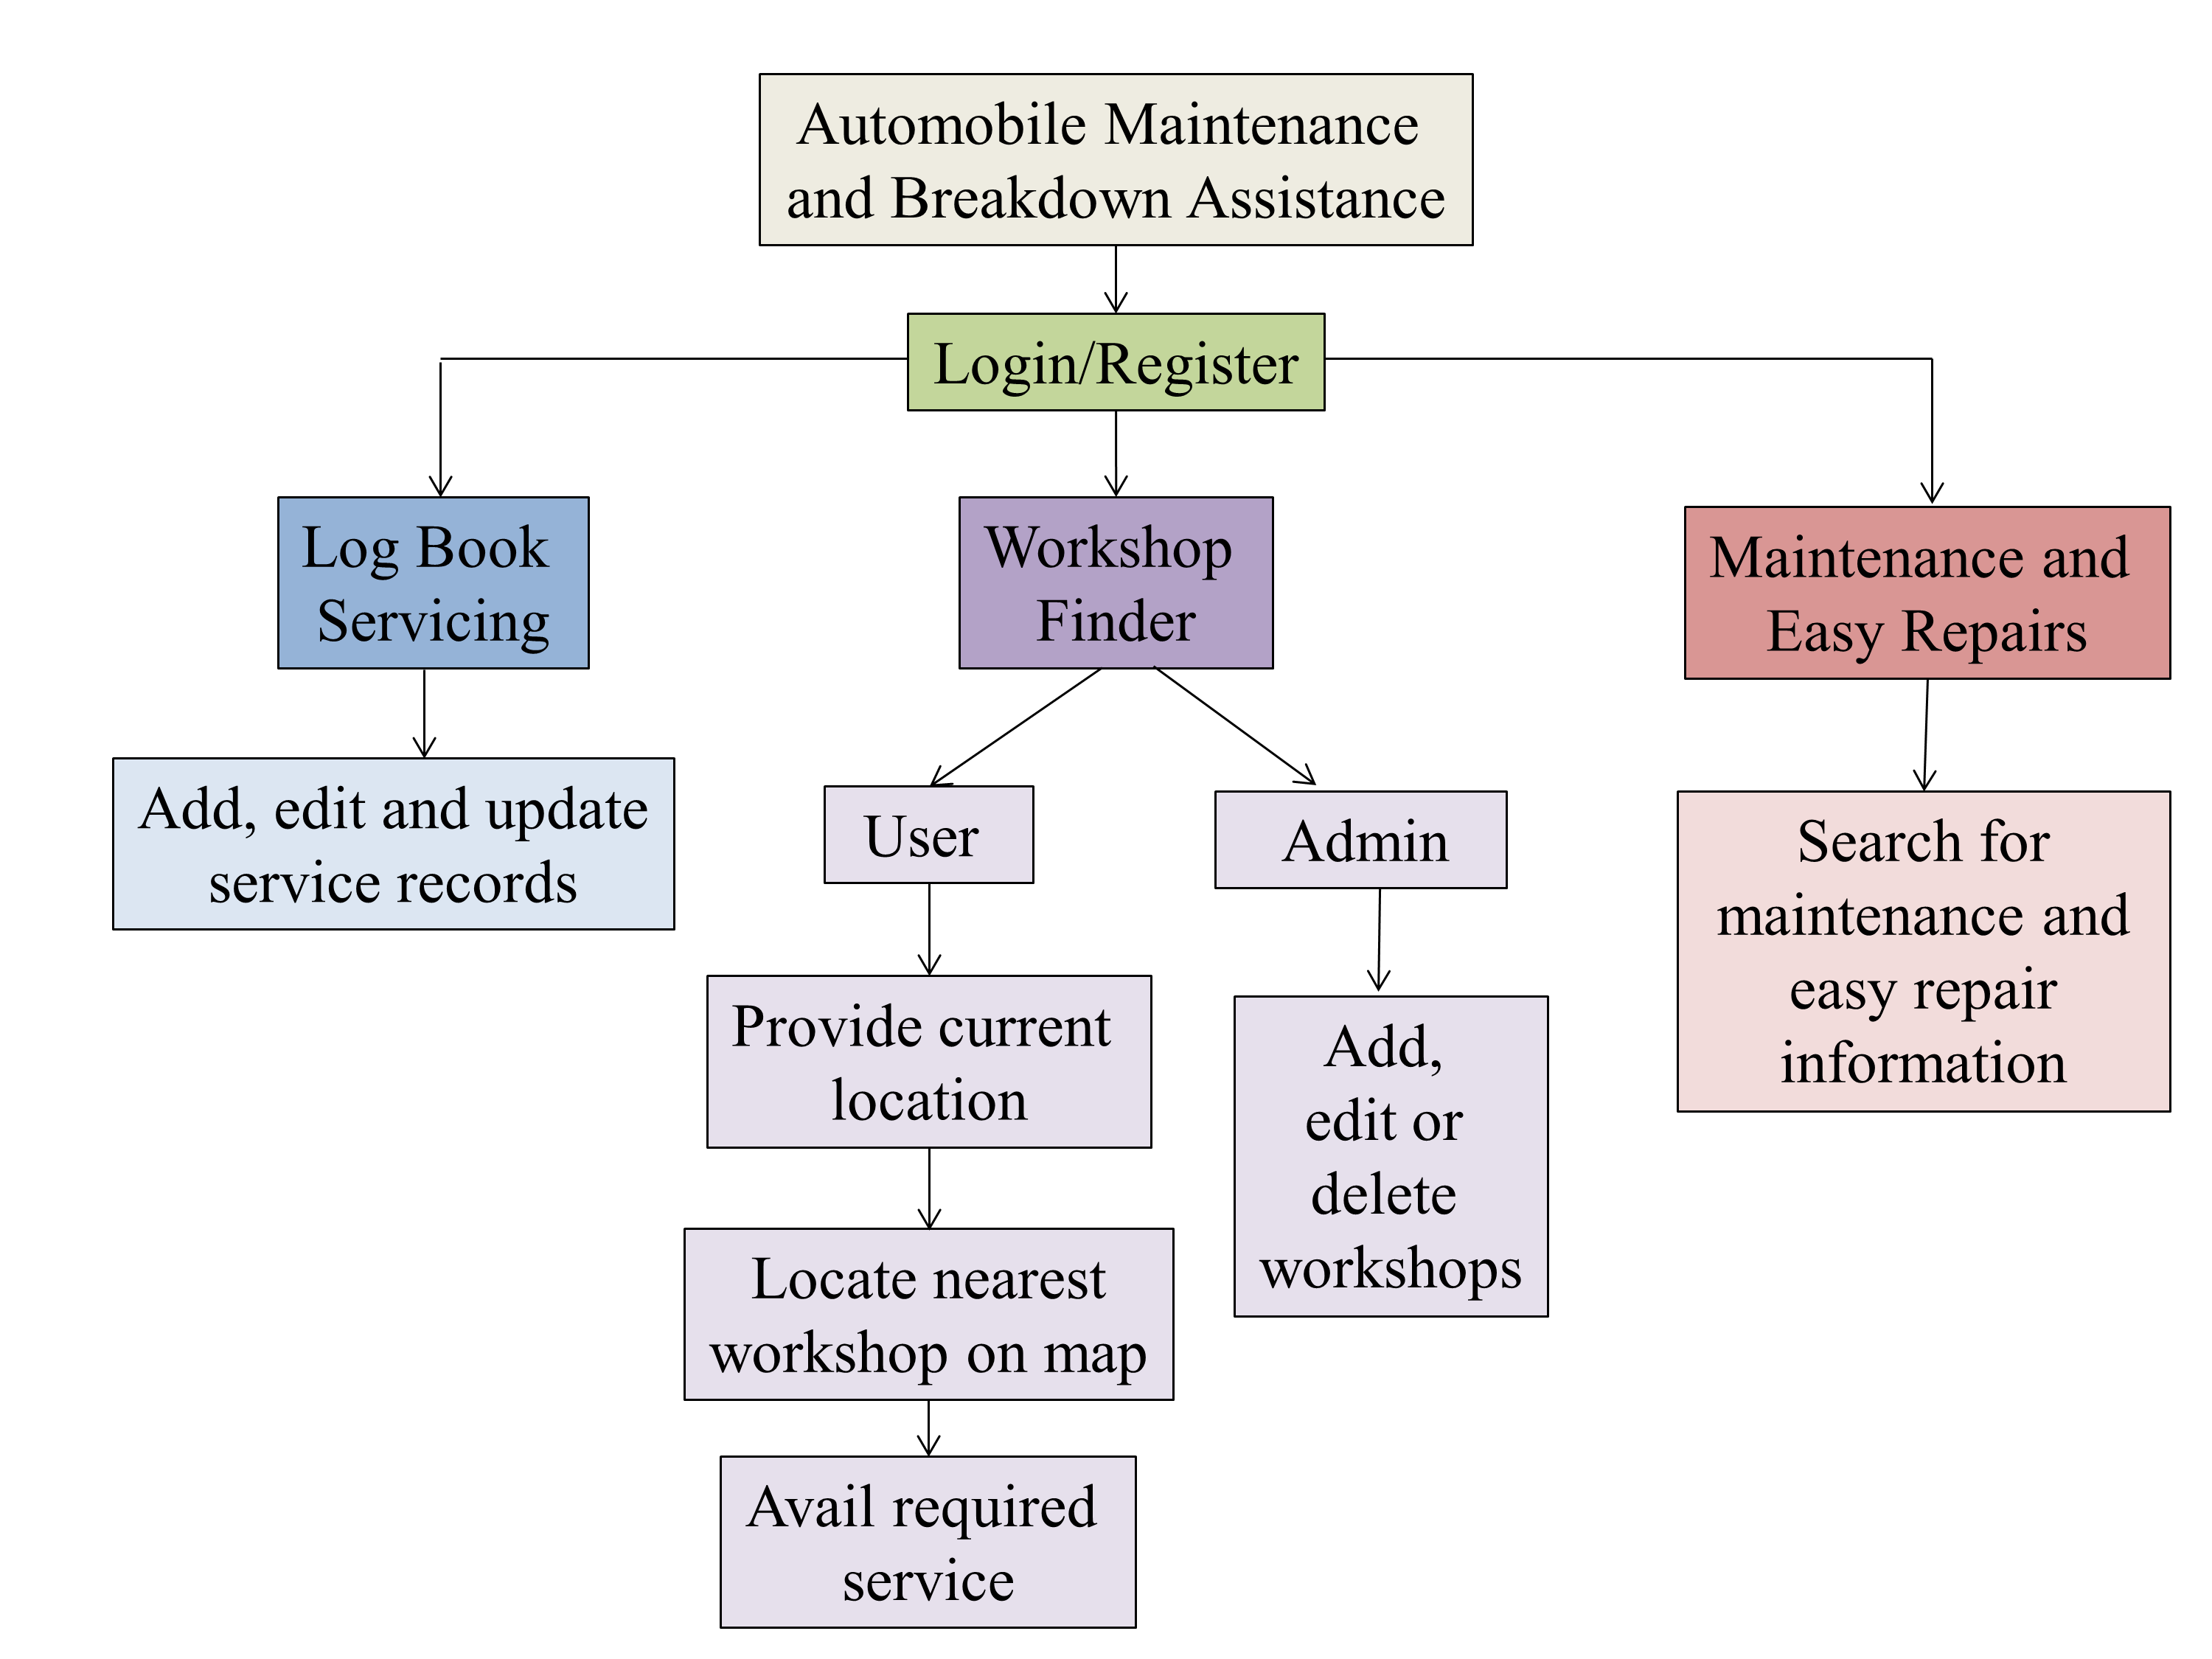
\includegraphics[width=\linewidth]{overview.png}\par 
        \caption{Overview of automobile maintenance and breakdown assistance}
        \label{fig:overview}
    \end{figure}
	This web app has three core functionalities: 1) Log book servicing 2) Workshop finder and 3) Maintenance and easy repair information. 
	Users has to register their basic details like username, password, email, etc to obtain access to these services. Once registered, they can login and avail service whenever needed.\\
	The log book servicing module is used to keep track of the users' vehicle maintenance and service record. Attributes include the make, model, type (gas, diesel or electric), year, odometer reading and maintenance task performed such as, oil change, tire rotation, wheel change, etc. This module supports the CRUD (Create, Read, Update and Delete) concept by creating new service record, reading the existing ones, updating new maintenance records and deleting existing ones. This log book service is a dynamic approach to proper car maintenance where regular inspections and small fixes are recorded to ensure smooth and efficient running of vehicles.\\
	The workshop finder module is controlled by an admin. The admin provides approval and registers mechanics and workshops to the website obtaining required information about their exact location and contacts. These locations are integrated to the map of the website. While the user, can track workshops nearest to his location and call for help in case of breakdown or vehicle malfunction.\\
	Maintenance and easy repair information are also provided which would aid the user in providing a temporary and easy backup solution to keep his vehicle running for the time being performing some DIY (do it yourself) bug fixes.\\
	In a word, our web application has been developed with the sole purpose of ensuring smooth and uninterrupted journey anywhere by regularly inspecting and updating maintenance record of vehicles and providing prompt mechanic service from the nearest location in case of mechanical failure.
	\subsection{Structure of the document}
	The document is structured as follow:
	\begin{itemize}
	\item Section 2, provides an overview of the entire project management plan including project organization, process model used, hardware and software requirements and estimated budget with proper risk analysis. 
	\item Section 3, describes the requirement specifications including different diagrams with graphical and textual descriptions. 
	\item Section 4, contains the overall model architecture along with the hardware and software technology implemented to build it.
	\item
	Section 5, represents the component level design and graphical user interface (GUI) design. \item Section 6, provides testing of the application and describes a sustainability plan for future updates and configurations.
	\end{itemize}
	
	\subsection{Terms, Acronyms, and Abbreviations Used}
	\textbf{CRUD} - Create, Read, Update and Delete\\
	\textbf{SDLC} - System Development Life Cycle\\
	\textbf{GUI} - Graphical User Interface\\ \textbf{API} - Application Programming Interface\\
	\textbf{RMMM} - Risk Mitigation, Monitoring and Management\\
	\textbf{IDE} - Integrated Development Environment\\
	\textbf{MVC} - Model-View-Controller.
	
\section{Project Management Plan}
	\subsection{Project Organization}
	Project Organization and responsibilities were distributed between the team members and their individual responsibilities are motioned in the following section. 
	
	\subsubsection{Individual Contribution to the project }
	
	Our team consists of three members and each member had their specified tasks to perform that contributed to the system development. A list of specified tasks performed by each member is mentioned in table \ref{tab:contribution}.
    \begin{table}[ht]
    \caption{Project Contributions}
    \begin{center}
    
    \label{tab:contribution}
    \begin{tabular}{ | c | c | c| }
    
    \hline
    \textbf{Team Member name} & \textbf{Student ID} & \textbf{Contribution to the project}\\
    
    \hline
    Adrita Barua & 1504015 & \begin{tabular}[c]{@{}c@{}} Conceptualization and initial planning of the project steps and\\ requirements. Coding and implementing the maintenance log,\\ search engine generation to retrieve repairing information \\and designing additional workshop finder module with \\back-end integration. Documentation and evaluation. \end{tabular}\\ 
    \hline
    Faria  Zarin Subah  & 1504027 & \begin{tabular}[c]{@{}c@{}} Planning and analysis of the design steps. Ensuring\\ requirement specification and feedback analysis.\\ Programming and integrating the OpenStreetMap with the \\Workshop Finder module and implementing cloud server database\\ connection. Scheduling and process estimation. \end{tabular}\\
    \hline
    Tarek Hossain & 1504014 &\begin{tabular}[c]{@{}c@{}}  Defining System Architectural pattern and monitoring\\ design steps. User interface design and implementation. \\Performance evaluation and risk analysis.
    \\Debugging and test case generation.\end{tabular}\\
    \hline
     
    \end{tabular}
    \end{center}
    \end{table}
    
	\subsection{Process Model Used}
	A Process model is structured to define a specific road-map that brings order to the chaos of software development. A well defined process model is required to provide stability, control and organization to avoid too much chaos but at the same time modern process models should be "agile". So, to ensure the quality, timelessness and long term viability of the product, the importance of an efficient process model is inevitable. The workflow of all the activities should be guided by the process steps as well as there should be scope of development accordingly to the changing requirements of the software world. An iterative and responsive model should be the best fit to ensure the agile nature of software development models. In our project we've chosen the concurrent development model as our process model due to its iterative and concurrent development nature.   
	\begin{figure}[!hbt]
		 \centering
        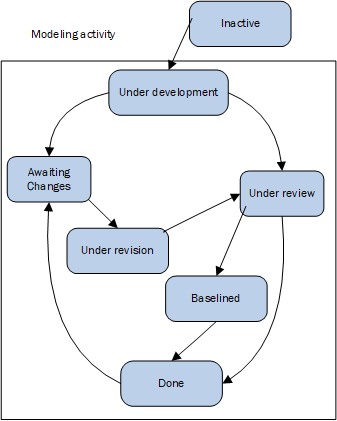
\includegraphics[width=10cm, height = 8.2cm]{process model.png} \par 
        \caption{Concurrent Process Model}
        \label{fig:process model}
    \end{figure}
		\subsubsection{Rationale for choosing your life-cycle model }
		Concurrent Model is used as the life-cycle model of our project because it provides an accurate picture of the current state of a project. It can be schematically defined as a  process network where all the software engineering activities exists simultaneously but in different states. This model overcomes the lengthy time consuming process of a spiral model and ensures the incremental speed by defining a series of events that triggers transitions from state to state for each of the actions or tasks. Figure \ref{fig:process model} shows an example of the concurrent modeling approach.


	    As an example, when the project completes its first iteration during the communication activity, it exists in the awaiting changes state. Now the modeling activity makes an transition to the under development state. However, if the customer makes an change in the requirements the modeling activity moves from the under development state to the awaiting changes state. Thus the concurrent model is used to ensure a process that facilitates flexibility, extensibility and speed of development.
	
	\subsection{Risk Analysis}
	Risk Analysis and management is the process that helps a software team to identify and manage potential problems that might occur in future due to uncertain circumstances.
	
	It can be defined as a three step process:
	\begin{itemize}
	    \item Identifying the risks
        \item Analyzing the impact of each identified risk
        \item Taking counter measures for the identified \& analyzed         risk
	\end{itemize}
	
	A risk analysis and management chart of our project is shown in table \ref{tab:risk analysis}. 
    
    \begin{table}[ht]
    \caption{Risk Analysis and Management table}
    \label{tab:risk analysis}
    \begin{center}
    
    \begin{tabular}{|c|c|c|c|}
    \hline
    \textbf{Risks} & \textbf{Probability} & \textbf{Impact} & \textbf{RMMM}
    \\ \hline
    
    \begin{tabular}[c]{@{}c@{}}Inaccurate scheduling and\\ estimation of development time. \end{tabular}
    & 40\% & 3
    & \begin{tabular}[c]{@{}c@{}}The team have to be more involved in\\ planning and estimating and try to get\\ early feedback from the stakeholders.\end{tabular}
    \\ \hline
    	
    \begin{tabular}[c]{@{}c@{}}Breakdown of requirement \\specification due to complex and \\unclear user requirements. \end{tabular}
    & 60\% & 2 
    & \begin{tabular}[c]{@{}c@{}}Use a iterative and well communicative\\ process model for early evaluation\\ of the system prototype. \end{tabular} 
    \\ \hline
    
    \begin{tabular}[c]{@{}c@{}}Taking a wrong and faulty \\design for a component or\\ system architecture. \end{tabular} 
    & 30\% & 2
    & \begin{tabular}[c]{@{}c@{}}Evaluate and research with detailed\\ information of different system\\ architecture during the planning. \end{tabular} 
    \\ \hline
    
    \begin{tabular}[c]{@{}c@{}}Technical risks occurred by using\\ new and evolving tools, \\techniques, protocols and \\development systems . \end{tabular} 
    & 70\% & 3
    & \begin{tabular}[c]{@{}c@{}}Proper training and skill development \\before using any new technology \\ can mitigate the technical risks. \end{tabular} 
    \\ \hline
    
    \begin{tabular}[c]{@{}c@{}}Failure to meet user \\ expectation on performance . \end{tabular} 
    & 60\% & 2
    & \begin{tabular}[c]{@{}c@{}} Proper benchmarks and threshold \\testing throughout the project have\\ to be implemented to ensure that\\ the work products are moving \\in the right direction. \end{tabular} 
    \\ \hline
    
    \end{tabular}
    \end{center}
    \end{table}
    
    \textbf{Impact Values used in the table}:
   
        \textbf{1} - catastrophic,
        \textbf{2} - critical,
        \textbf{3} - marginal,
        \textbf{4} - negligible,
 
	\subsection{Constraints to project implementation}
	
	\textbf{Software and Hardware constraints : }
	
	1. Google Map integration permission was restricted that occurred during system implementation.\\
	2. Some development tools were not supported due to poor hardware constraints.
	
	
	\textbf{Schedule and Budget constraints : }

	1. Project timeline schedule was disturbed due to the pandemic and other uncertain events.\\
	2. Due to poor budget, permission of Google map integration couldn't be accessed. 


	\subsection{Hardware and Software Resource (Tools/Language) Requirements}
	\vspace{.5cm}
	\textbf{Hardware Requirements:}
	\begin{itemize}
	\item Processor: Minimum 1 GHz; Recommended 2GHz or more
    \item Ethernet connection (LAN) OR a wireless adapter (Wi-Fi)
    \item Hard Drive: Minimum 32 GB; Recommended 64 GB or more
    \item Memory (RAM): Minimum 1 GB; Recommended 4 GB or above
    \end{itemize}
    \vspace{.5cm}
    \textbf{Software Requirements:}
    \begin{itemize}
        \item Front-End: HTML, JavaScript, CSS, Bootstrap
        \item Back-end: Node.js for server, mongoose for database connection, Robo 3T for database manipulation
        \item IDE: Visual Studio Code
        \item MongoDB Atlas, a global cloud database service used for data storage
        \item OpenStreetMap used for displaying map on the application.
    \end{itemize}
	
	\subsection{Project Timeline and Schedule}
	\begin{figure}[!hbt]
        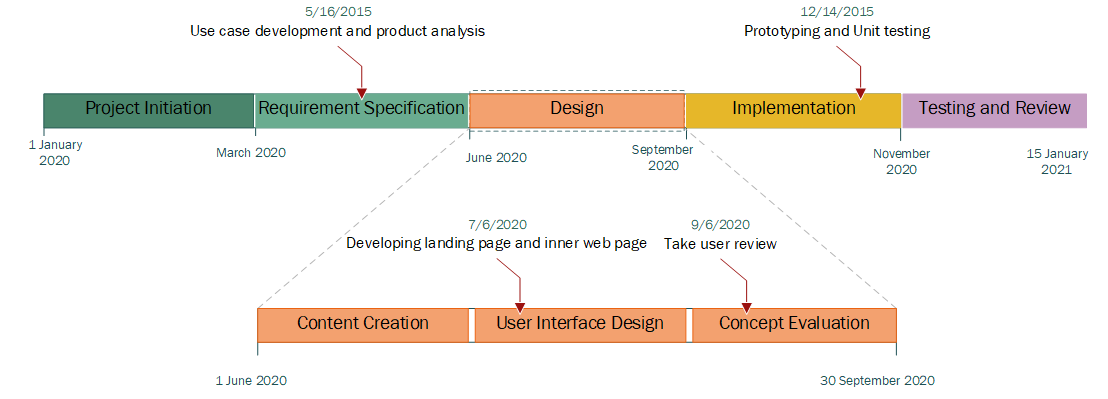
\includegraphics[width=\linewidth]{timeline.png}\par 
        \caption{Project Timeline and Schedule}
        \label{fig:timeline}
    \end{figure}

	\subsection{Estimated Budget}
	\begin{itemize}
	    \item Active Broadband Connection for one year : 30,000 BDT
	    \item 64 GB Hard Drive : 5,000 BDT
	    \item 4 GB RAM : 2,000 BDT
	\end{itemize}
    So, the total estimated budget was 37,000 BDT.
	\subsection{Social/Cultural/Environmental impact of the project}
	The rapid growth of population and their socio-economic solvency leads towards a huge market of Automobile servicing industry. Now a days almost every next person owns a personal vehicle that requires continuous maintenance and emergency servicing. In this present era of World Wide Web everyone wants quick services within one click. In this case,
	\begin{itemize}
	\item Our website can be a one-stop service that will provide the users information about their nearest workshops and help them avoid any unwanted vehicle malfunction by notifying them about the required early maintenance services. 
	\item Any automobile manufacturing company can advertise their products through our website which will provide a profitable economic impact on the society.
	\item This service will also help to avoid any unwanted accidents when such vehicle malfunctioning occurs in an unfamiliar road, a deserted lane or at a remote area, especially for female drivers. 
	\item Thus, our online assistance system can prove to be a very effective solution to ensure a smoother and easier transportation experience for any person who owns a personal vehicle or drives one.   
	\end{itemize}
		
\section{Requirement Specifications}
	\subsection{Stakeholders for the system}
	According to Somerville et al. \cite{johnston1998requirements}, a stakeholder is defined as "anyone who benefits in a direct or indirect way from the system which is being developed". Each stakeholder has a different view of the system, achieves different benefits when the system is successfully  developed, and is open to different risks if the development effort fails. The stakeholders identified in our system are end users like owner of personal automobiles or an automobile company owner, administrator who will approve and add workshops belonging to different areas, workshop managers, fuel station managers and mechanics who will provide service to user vehicles, product engineers, software engineers and also support and maintenance engineers. 
	\subsection{Use case diagram with Graphical and Textual Description}
	A use case diagram depicts the software or system from the end user's point of view.
	The use case diagram of our software is depicted in Figure \ref{fig:usecase}.
	\begin{figure}[!hbt]
        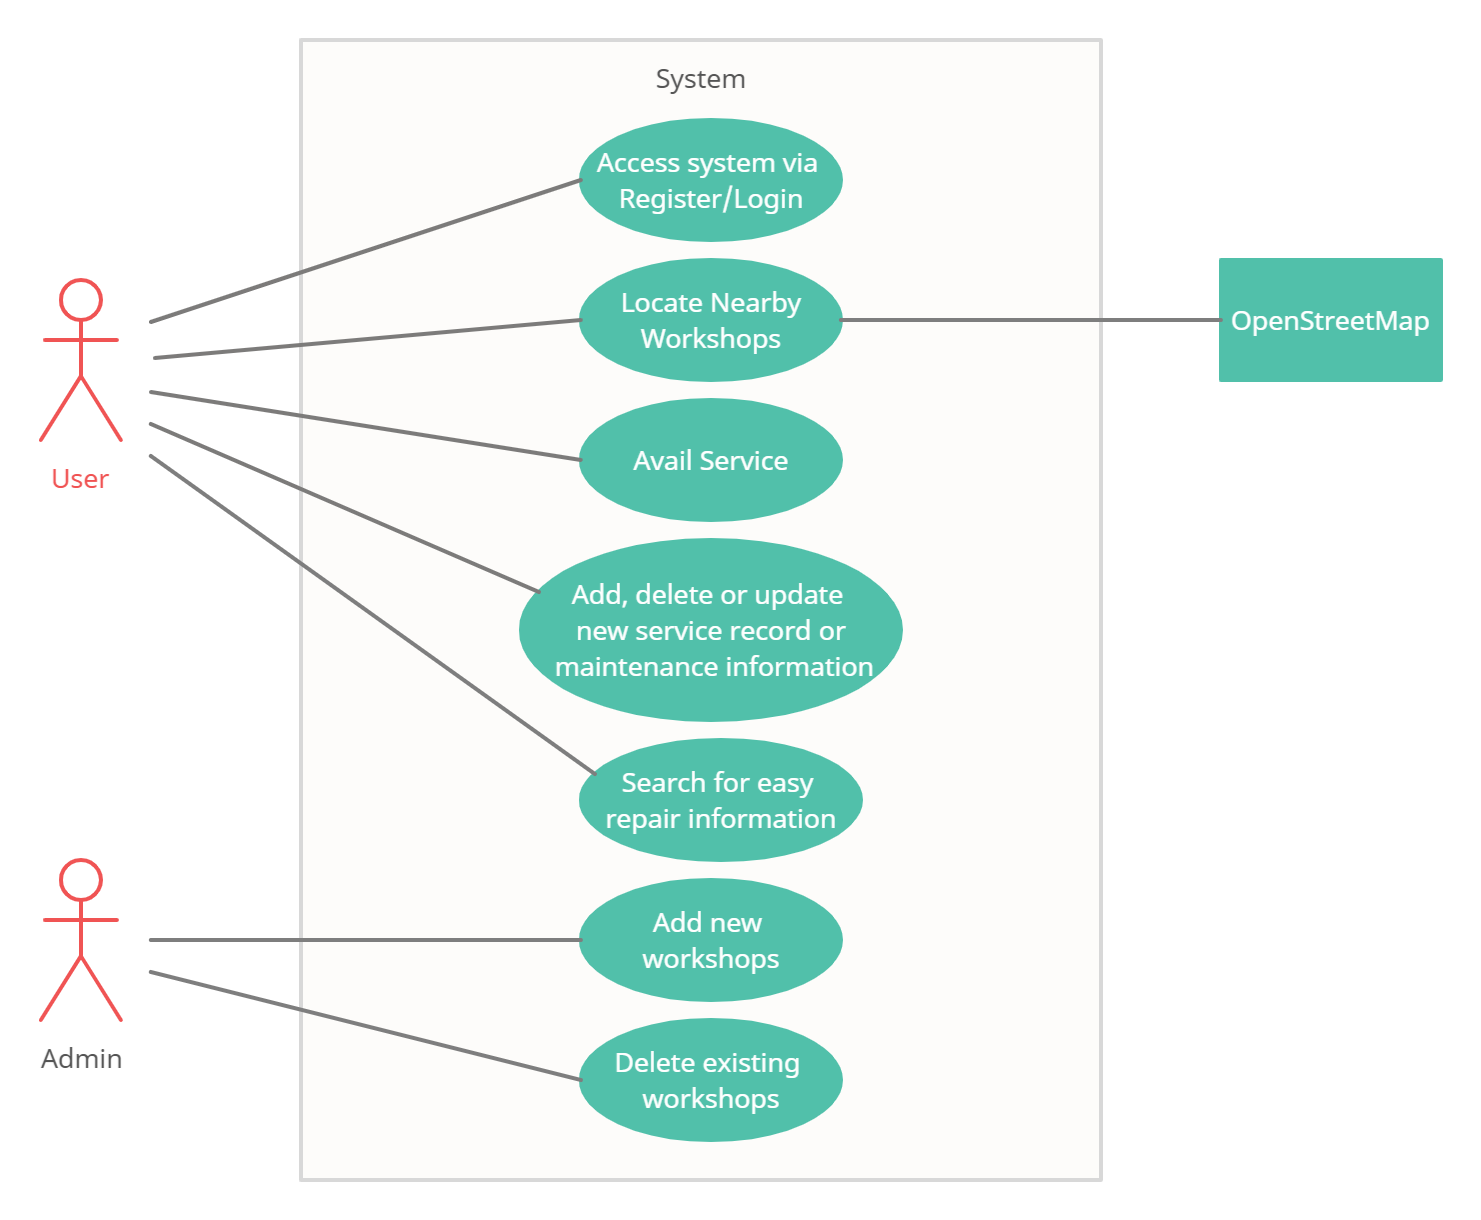
\includegraphics[width=15cm,height= 9cm]{Use Case.png}\par 
        \caption{Use Case Diagram}
        \label{fig:usecase}
    \end{figure}

	The textual description of the use-case diagram is represented following the template suggested by Cockburn et al. \cite{usecases}.
	\begin{enumerate}
	\textbf{Use Case:} \emph{AvailVehicleService} \\
	\textbf{Primary Actor:} User\\
	\textbf{Goal in context:} To locate and avail service from nearby workshops in case of vehicle breakdown \\
	\textbf{Preconditions:} User registers the system using required information. Admin approves and adds location of workshops around the area into the system.\\
	\textbf{Scenario:} \\
	1. User: Registers into the system\\
	2. User: Enters password and logs in\\
	3. User: Selects workshop finder and locates nearby workshops from his current location\\
	4. User: Avail service in case of vehicle repair by contacting nearby workshops\\
	5. User: Updates service log and maintenance records\\
	\textbf{Exceptions:}\\
	1. Password or username is incorrect (Wrong password or invalid username message is displayed): User reenters correct password or username\\
	\textbf{Priority:} Essential, must be implemented\\
	\textbf{Frequency of use:} Each time a vehicle breaks down or malfunctions and service is availed\\
	\textbf{Channel to actor:} Via GUI (graphical user interface)\\
	\textbf{Secondary actors:} Admin, OpenStreetMap\\
	\textbf{Channels to secondary actors:} \\
	Admin: Via Admin API (application programming interface)
	OpenStreetMap: Fetch and save raw geodata from/to OpenStreetMap database\\
	\textbf{Open-Issues:}\\
	1. Should there be a way to activate the system without the use of a password\\
	2. Should there be a way to gain a new password if previous password is forgotten by the user\\
	3. Should there be an added functionality using hardware devices like sensors to produce service alerts before the vehicle halts completely.
	\end{enumerate}
	
	\subsection{Activity Diagram:}
	The Activity Diagram of our system is shown in figure \ref{fig:Activity Diagram}
	
	\begin{figure}[!hbt]
		 \centering
        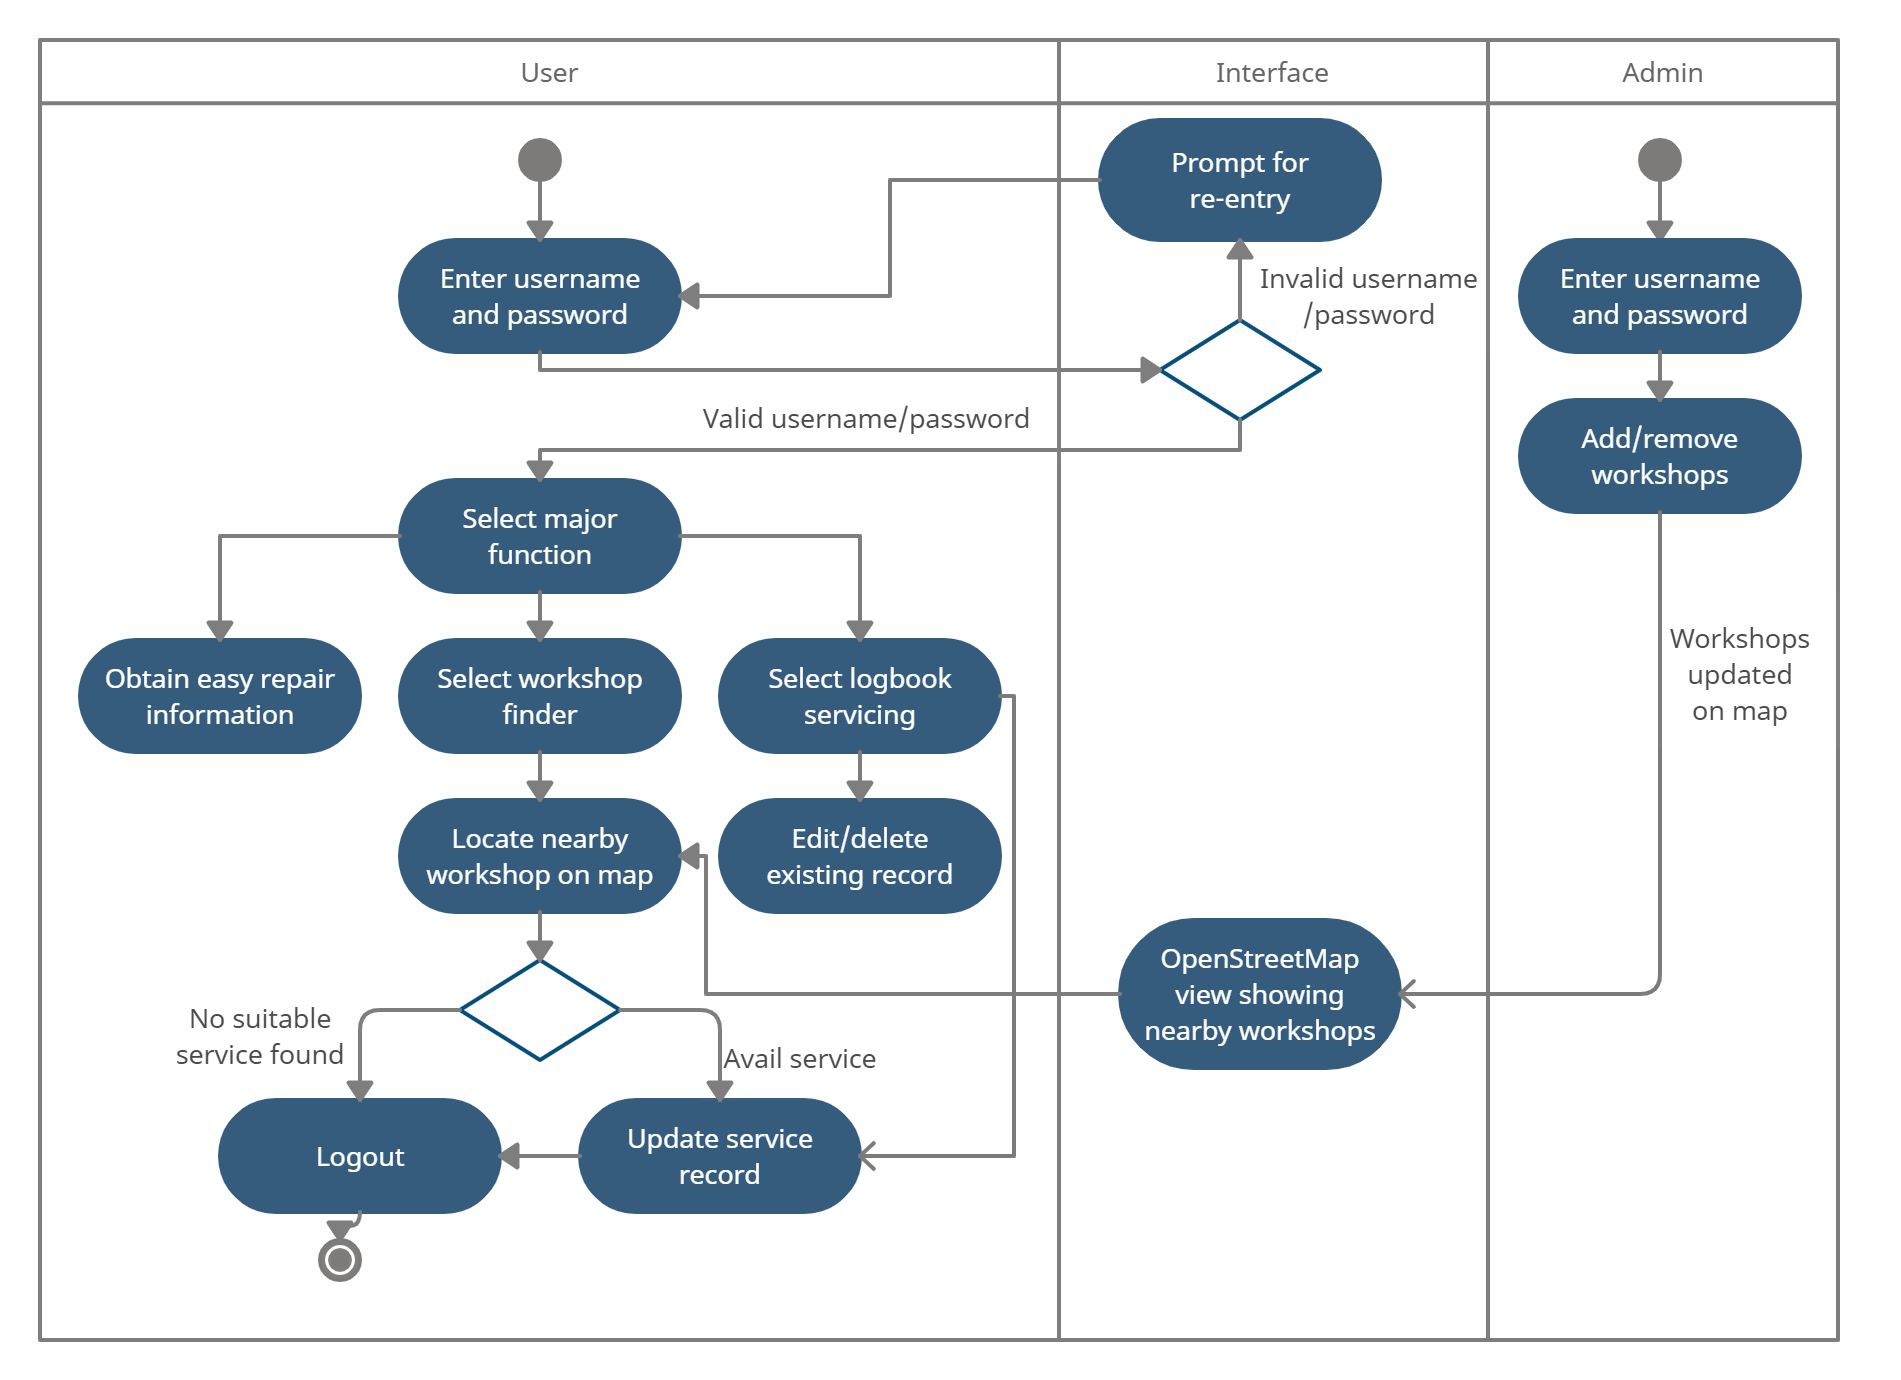
\includegraphics[width=15cm\textwidth]{Activity Diagram.png} \par 
        \caption{Activity Diagram}
        \label{fig:Activity Diagram}
        \end{figure}
	
	\\
	\subsection{Static model – class diagram:}
	The Class Diagram of our system is shown in figure \ref{fig:Class Diagram}
	
	
	\begin{figure}[!hbt]
		 \centering
        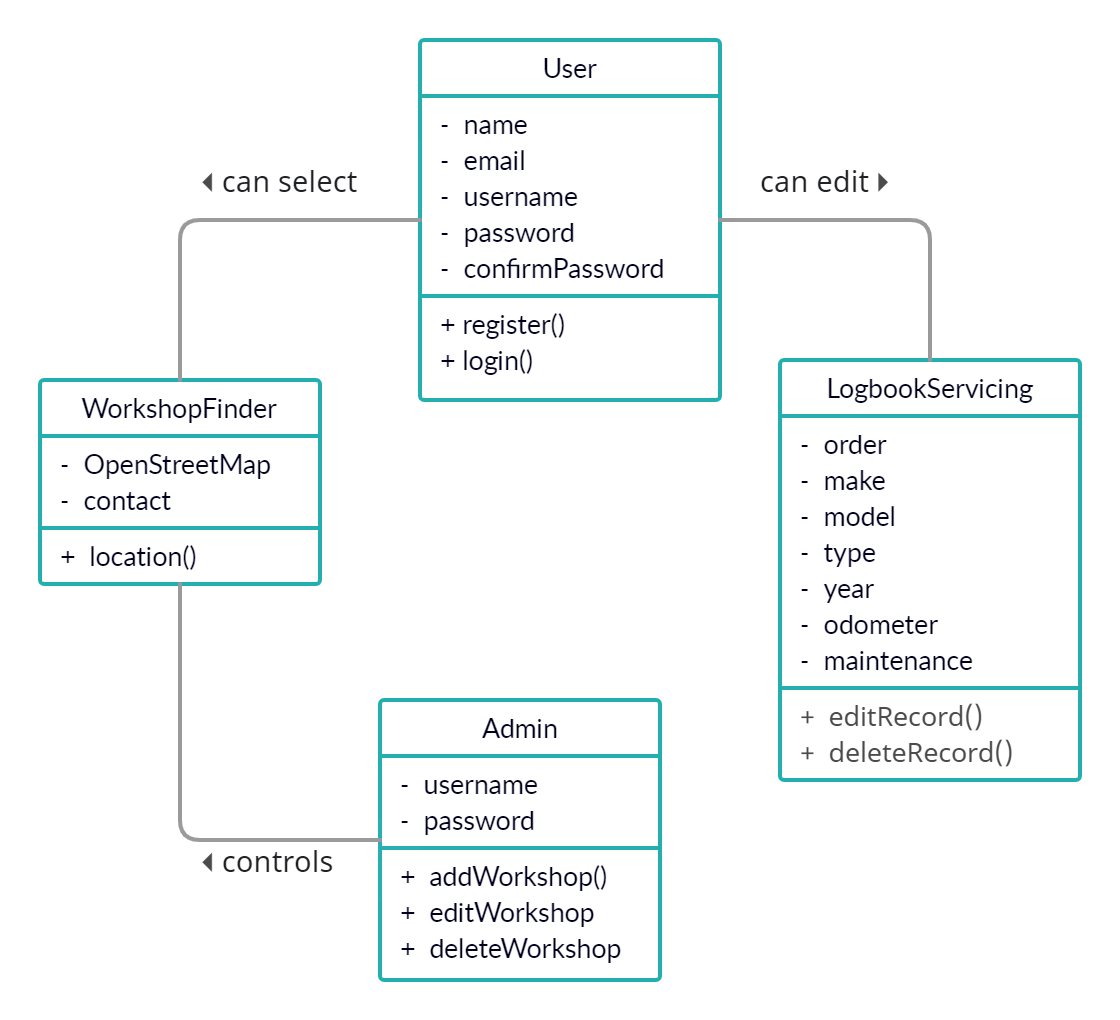
\includegraphics[width=15cm,height= 9cm]{Class Diagram.png} \par 
        \caption{Class Diagram}
        \label{fig:Class Diagram}
        \end{figure}
	
	\subsection{Dynamic model – sequence diagram:}
	
		
	\begin{figure}[!hbt]
		 \centering
        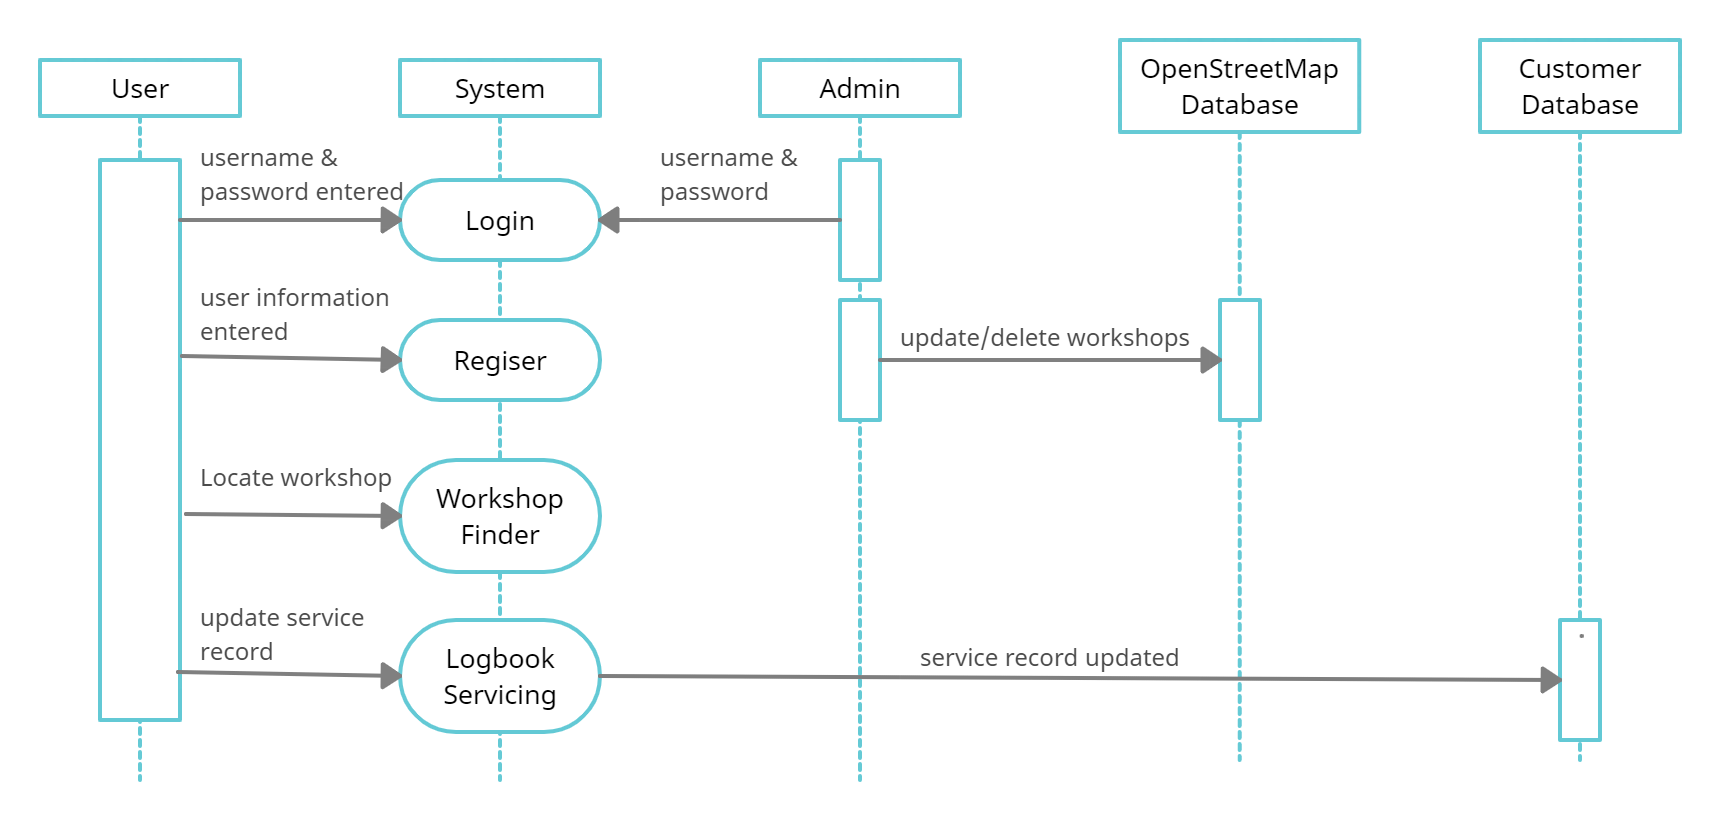
\includegraphics[width=15cm]{sequence diagram.png} \par 
        \caption{Sequence Diagram}
        \label{fig:Sequence Diagram}
        \end{figure}
	
	\subsection{Safety and Security requirements}
	Software security is an integral prerequisite for software reliability, safety and integrity. To determine the safety and security requirements of a particular software product it is required to identify the sensitive assets that has to be protected and the cost associated if a security breach occurs.
	
		\subsubsection{Access Requirements}
		Access requirement specifies who has authorized access to which part of the product and to what extent it is granted. In case of this product, admin has access only to the workshop finder functionality. Only the admin can add new workshops to the database and edit or delete existing ones. Users who visit the website without registering can only view the easy maintenance information page but cannot avail service. Registered users can locate nearby workshops to avail service and maintain a service record.
		\subsubsection{Integrity Requirements} 
		Integrity requirements categorize data/assets and determines what kind of data needs to be protected and validated when it already exists in the system or when communicating with external components. In our system, all sorts of user data has been saved to MongoDB Atlas database after getting encrypted at several levels. This cloud based database service protects data from disclosure. We care the privacy of user information and are dedicated to protect clients' privacy. Passwords are also encrypted and validated each time a user logs into the system. 
		\subsubsection{Privacy Requirements}
		No user data is handled to any third-party organization. This software product has been designed and deployed strictly adhering to the legal framework provided by information privacy or data protection laws.
	
\section{Architecture}
	\subsection{Architectural model/style used}
	An Architectural style establishes a structure for all the components of the system that is imposed on the design transformation. There are different architectural styles that are analyzed to derive the structure that is best suited to the system requirements and quality attributes.
	For our Web Application we have used Model-View-Controller(MVC) architecture \cite{archi}.
	
		\subsubsection{Rationale for choosing your architectural model/style}
		The architecture of a system describes the infrastructure that enables the systems or applications to required objectives. In our project we've built a web-app that provides vehicle assistance service which is designed based on the MVC architecture. This model is suggested to be one of the best suited architectures for Web-App development. It is a three layered design architecture that keeps interface, application and navigation separate from each other which simplifies implementation and enhance reuse. The first module or layer is named "Model" which contains all application-specific content, processing logic and all processing functionality that is application specific. The "View" contains all interface-specific functions and enables the presentation of the
		content and processing logic and all processing functionality required by end user. The "Controller" manages access to the model and view and coordinates the data flow between them. A schematic representation of the MVC architecture is shown in Figure \ref{fig:MVC}
		\begin{figure}[!hbt]
		\centering
        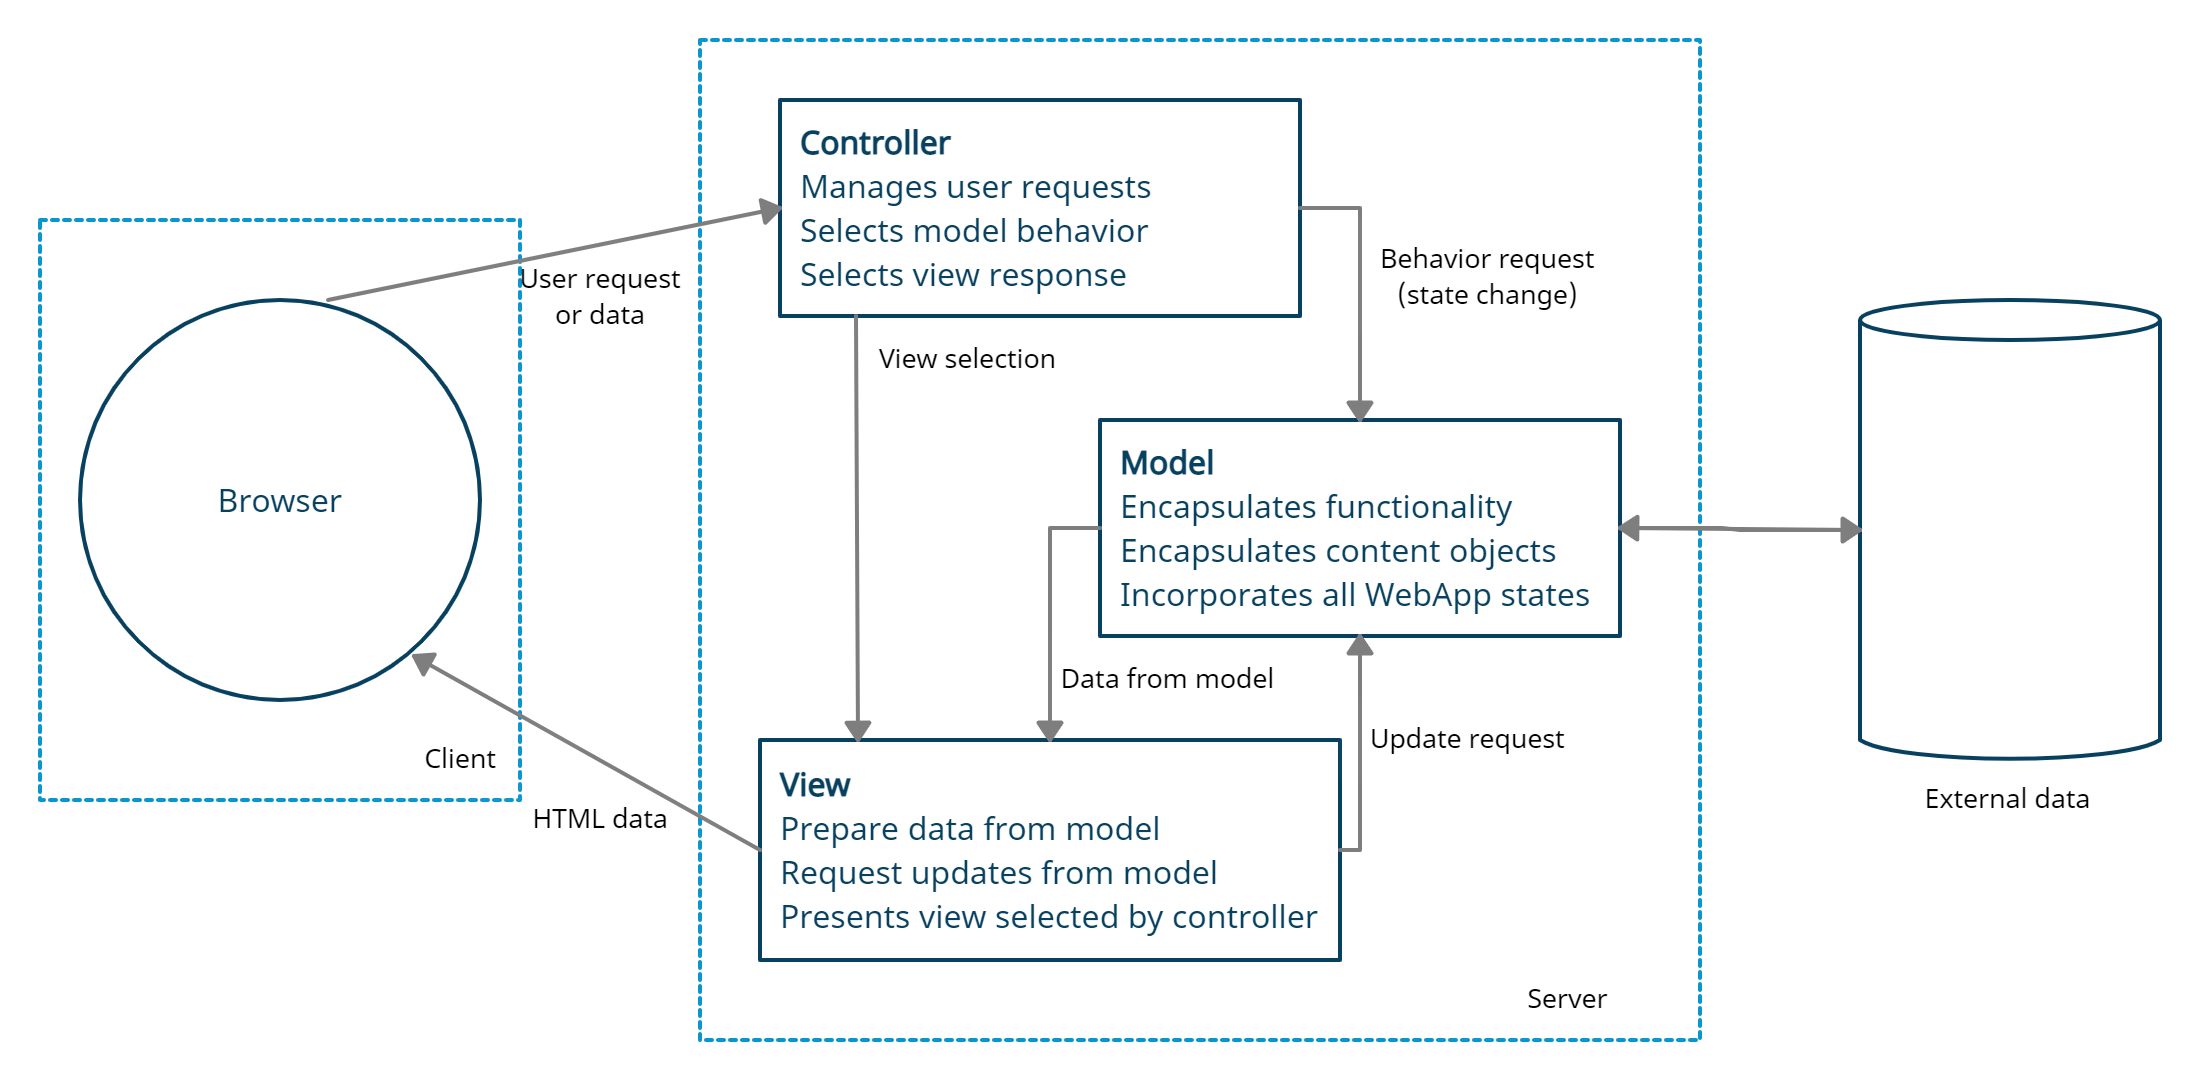
\includegraphics[width=\linewidth]{MVC.png} \par
        \caption{The MVC architecture}
        \label{fig:MVC}
    \end{figure}
		
		
	
	\subsection{Technology, software, and hardware used}	
	Personal Computers are used as the basic Hardware device to implement the system that includes 2GHz Processor and 4 GB RAM configuration.
	HTML, JavaScript, CSS, Bootstrap framework is used for Front-end development.In the Back-end Node.js is used for server, mongoose for database connection and Robo 3T is used for database manipulation. MongoDB Atlas, a global cloud database service used for data storage. OpenStreetMap used for displaying map on the application. Visual Studio Code is used as the coding tool.

\section{Design}
After completing the process of requirement analysis and modeling, software design is the final step within the modeling activity that prepares the system to enter the construction stage where code generation and testing takes place. The information flow from requirement modeling to design is illustrated in Figure \ref{fig:transleting diagram}. The requirement model manifested with use case diagram, activity diagram, sequence diagram and class diagram guides the design task. The component level design following pattern and interface design is illustrated in the subsequent sections.
	\begin{figure}[!hbt]
		\centering
        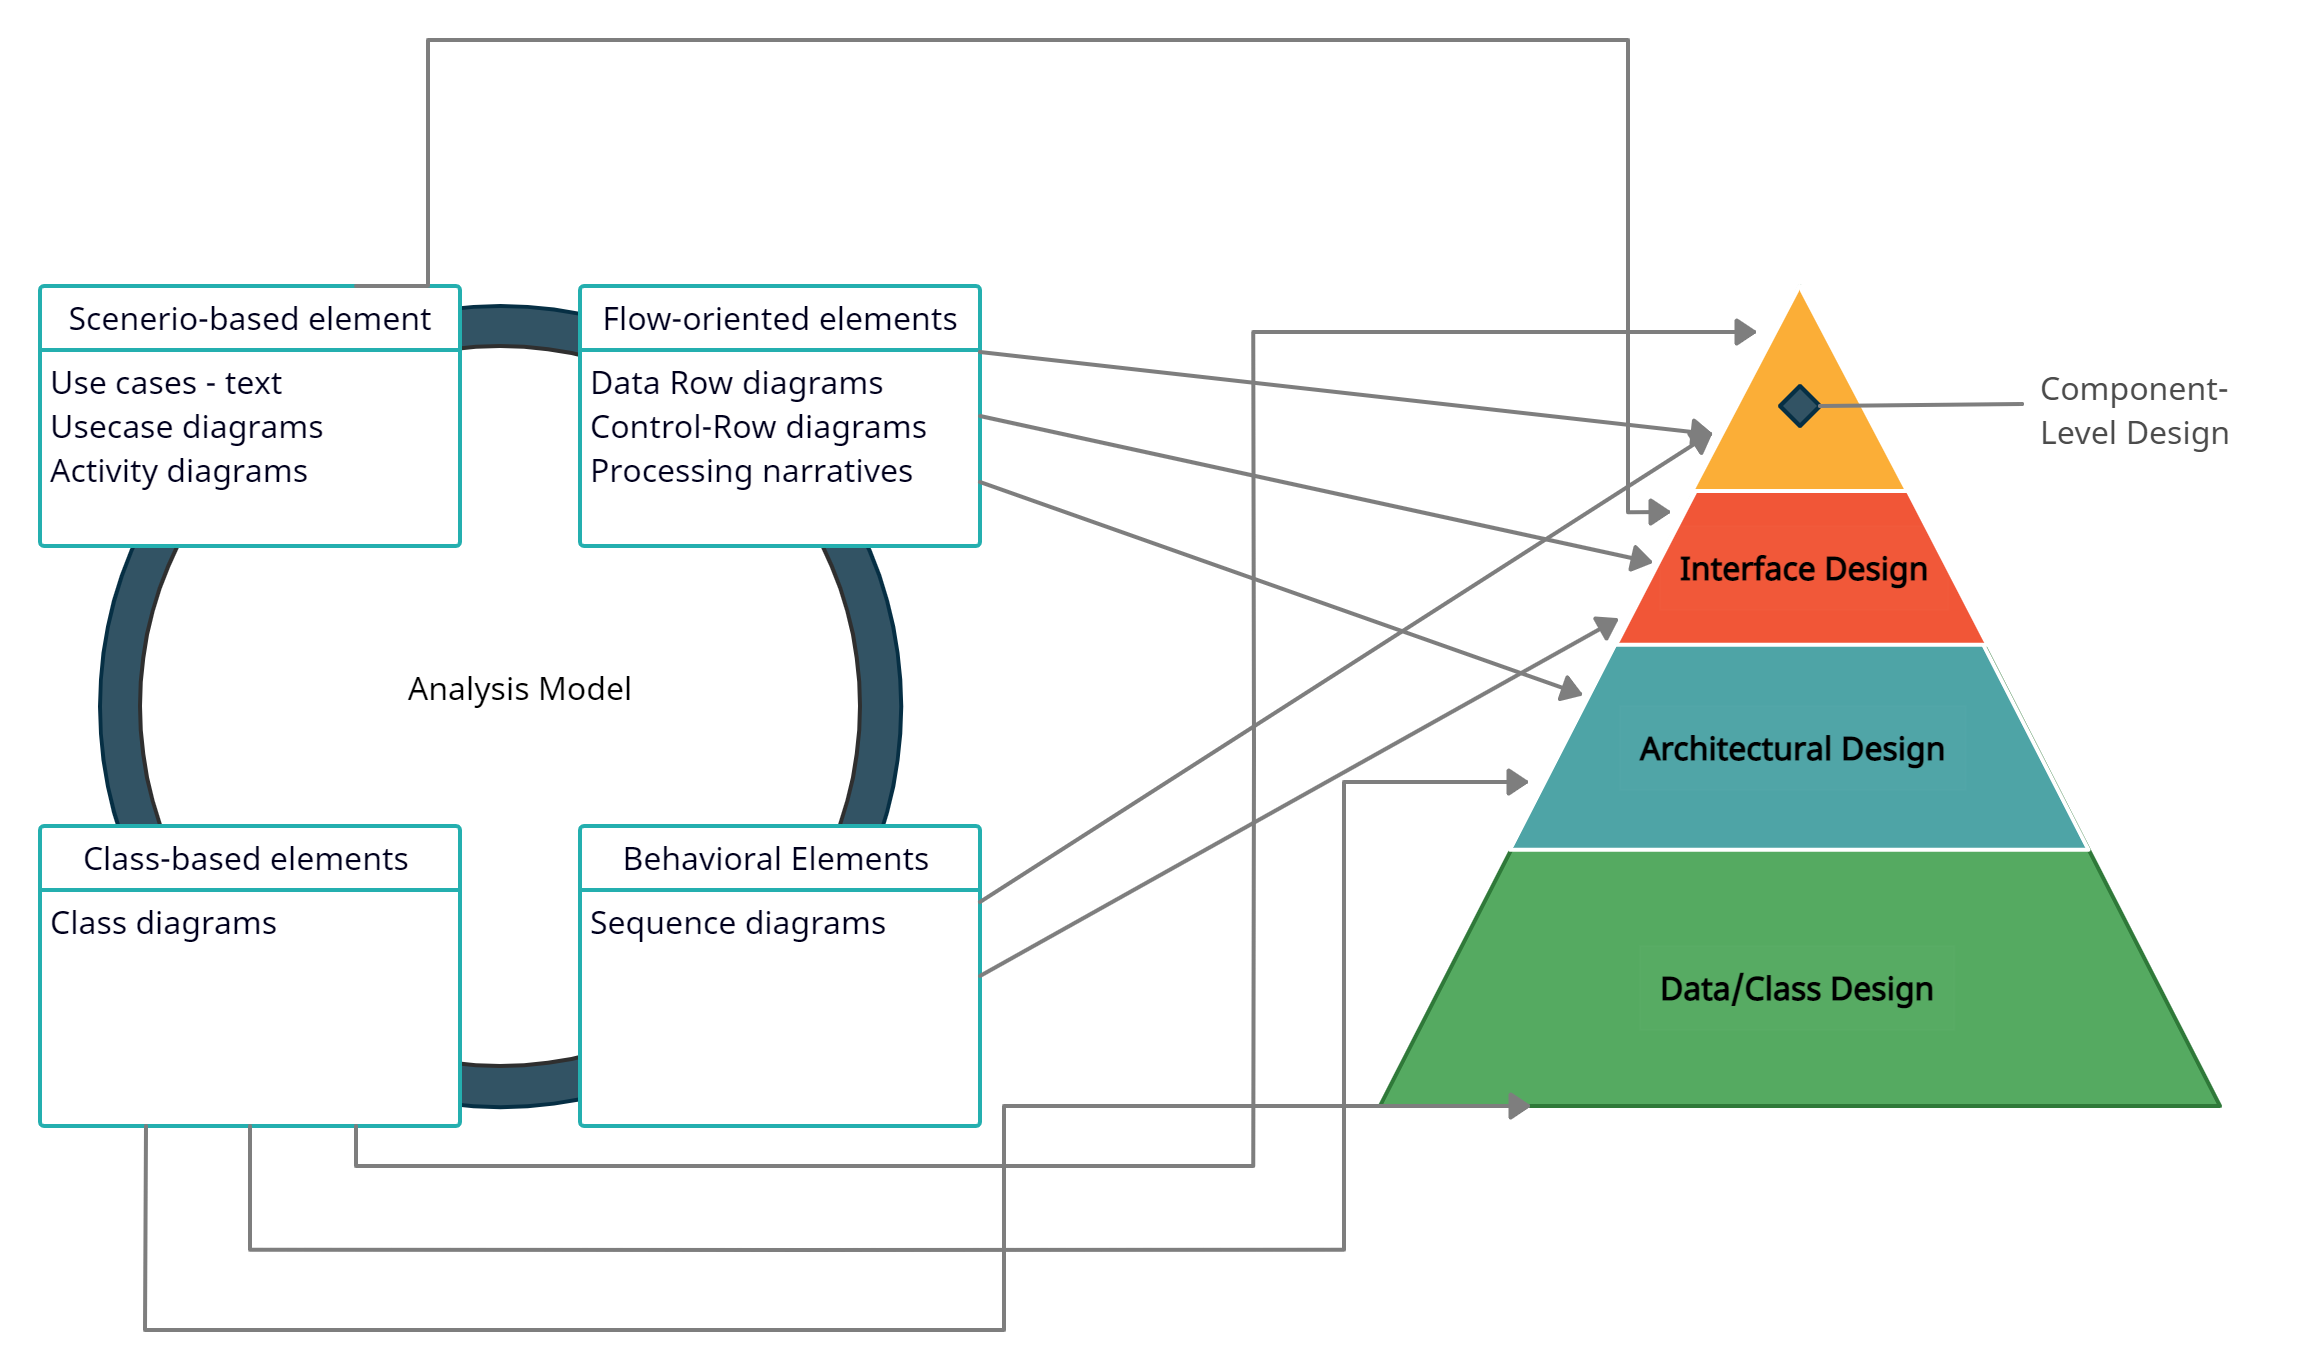
\includegraphics[width=\textwidth,height = 7.5 cm]{Translating the requirement model into the design model.png} \par 
        \caption{Translating the requirement model into the design model}
        \label{fig:transleting diagram}
    \end{figure}
	\subsection{Component level design following pattern}
    
	\begin{figure}[!hbt]
		\centering
        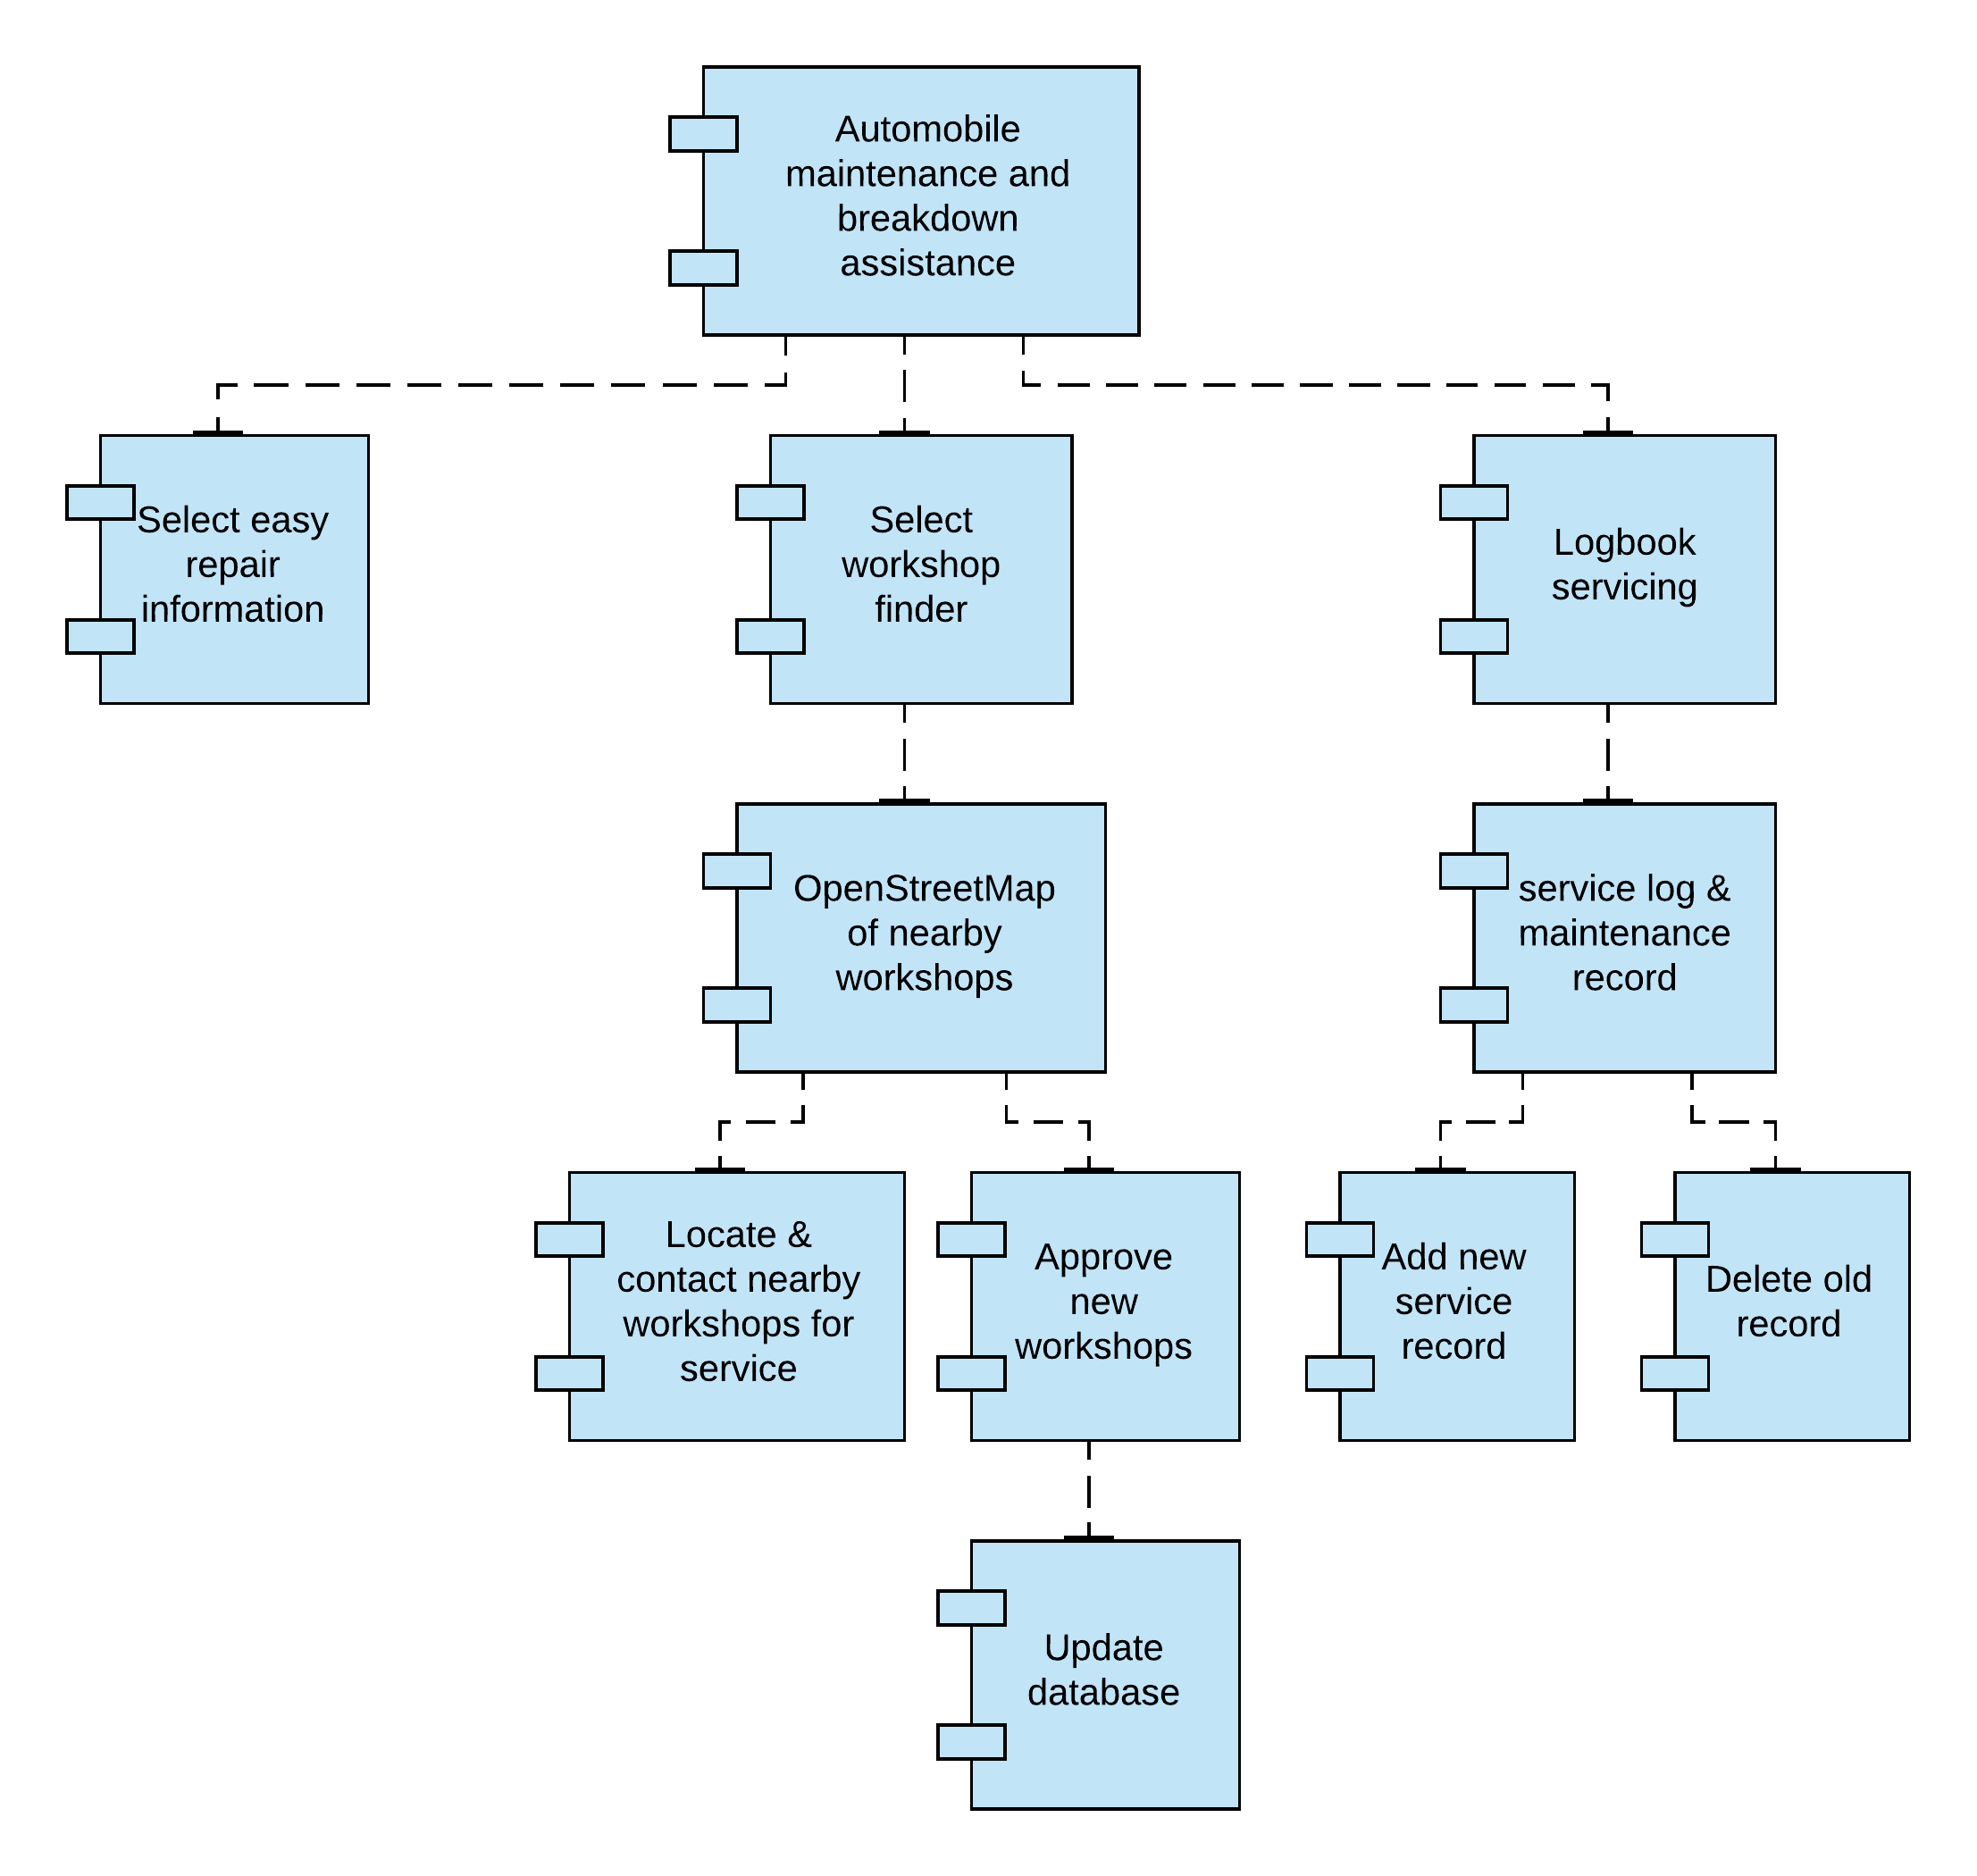
\includegraphics[width=12cm, height = 8.5cm]{Component Diagram.png} \par 
        \caption{Component Level Design}
        \label{fig:Component Diagram}
    \end{figure}
    
	\subsection{GUI (Graphical User Interface) design}
	The following figures represent the GUI design of our software product and provides and overview regarding how users can employ the functions and features offered by our Web-App.
	\begin{figure}[!hbt]
		\centering
        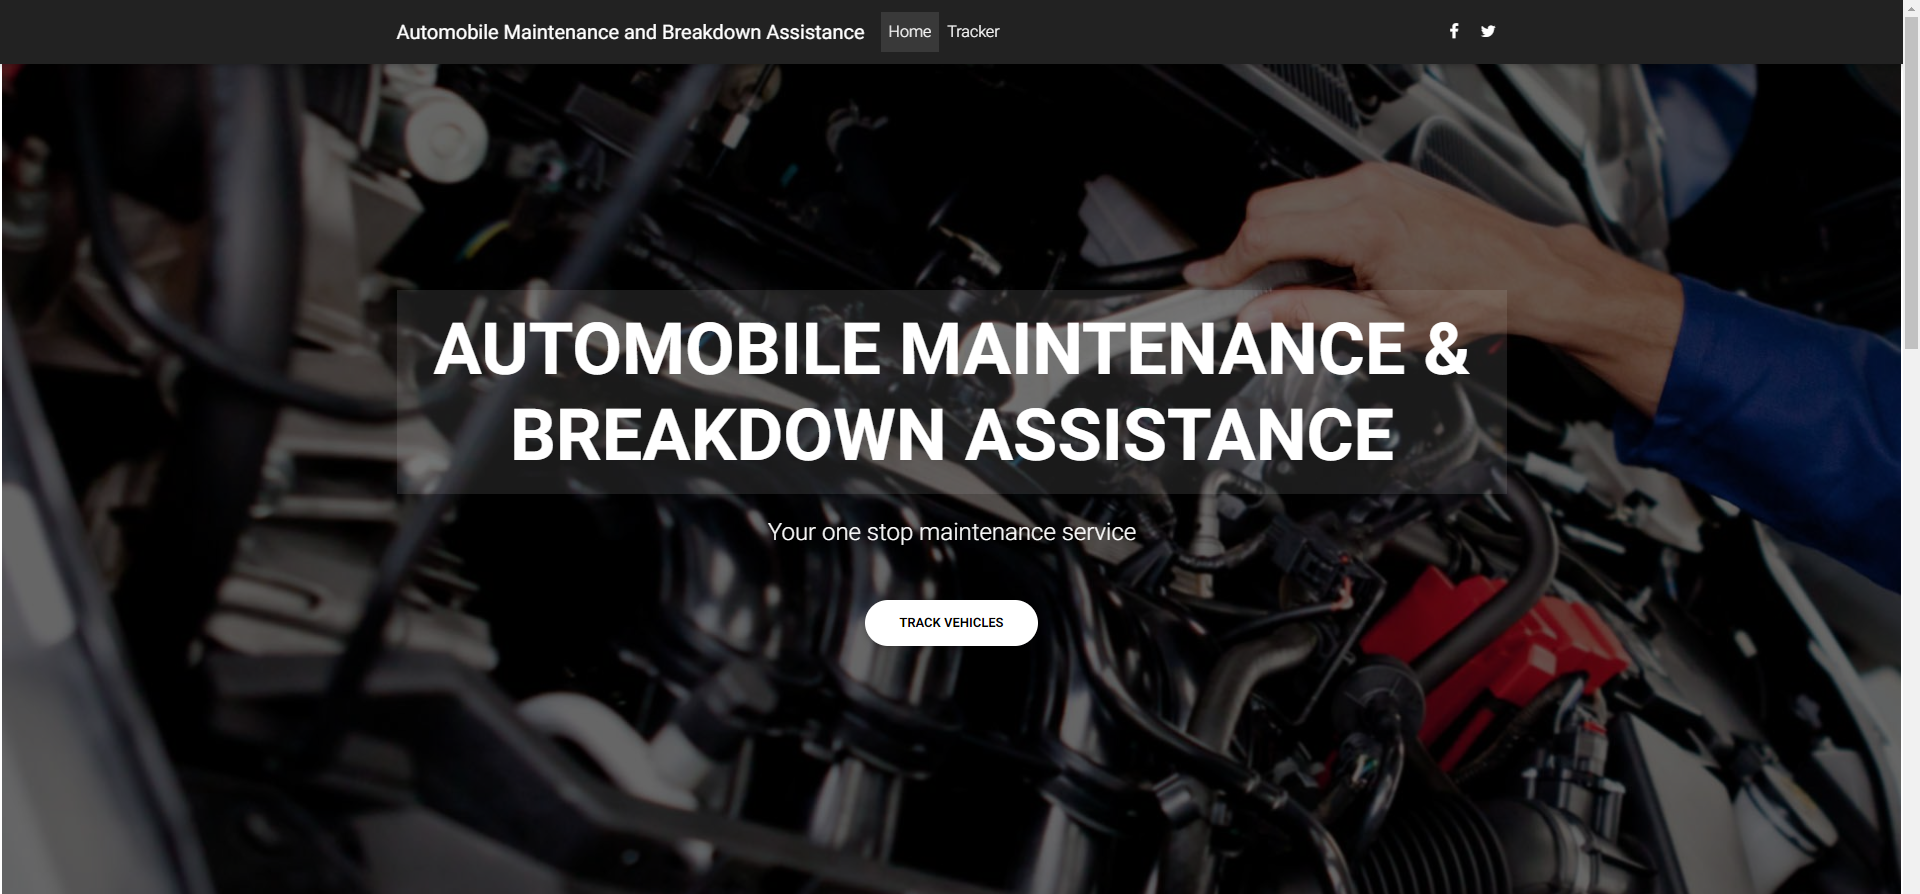
\includegraphics[width=15cm,height = 9cm]{home.PNG} \par 
        \caption{Home page}
        \label{fig:home page}
    \end{figure}
    
    \begin{figure}[!hbt]
		\centering
        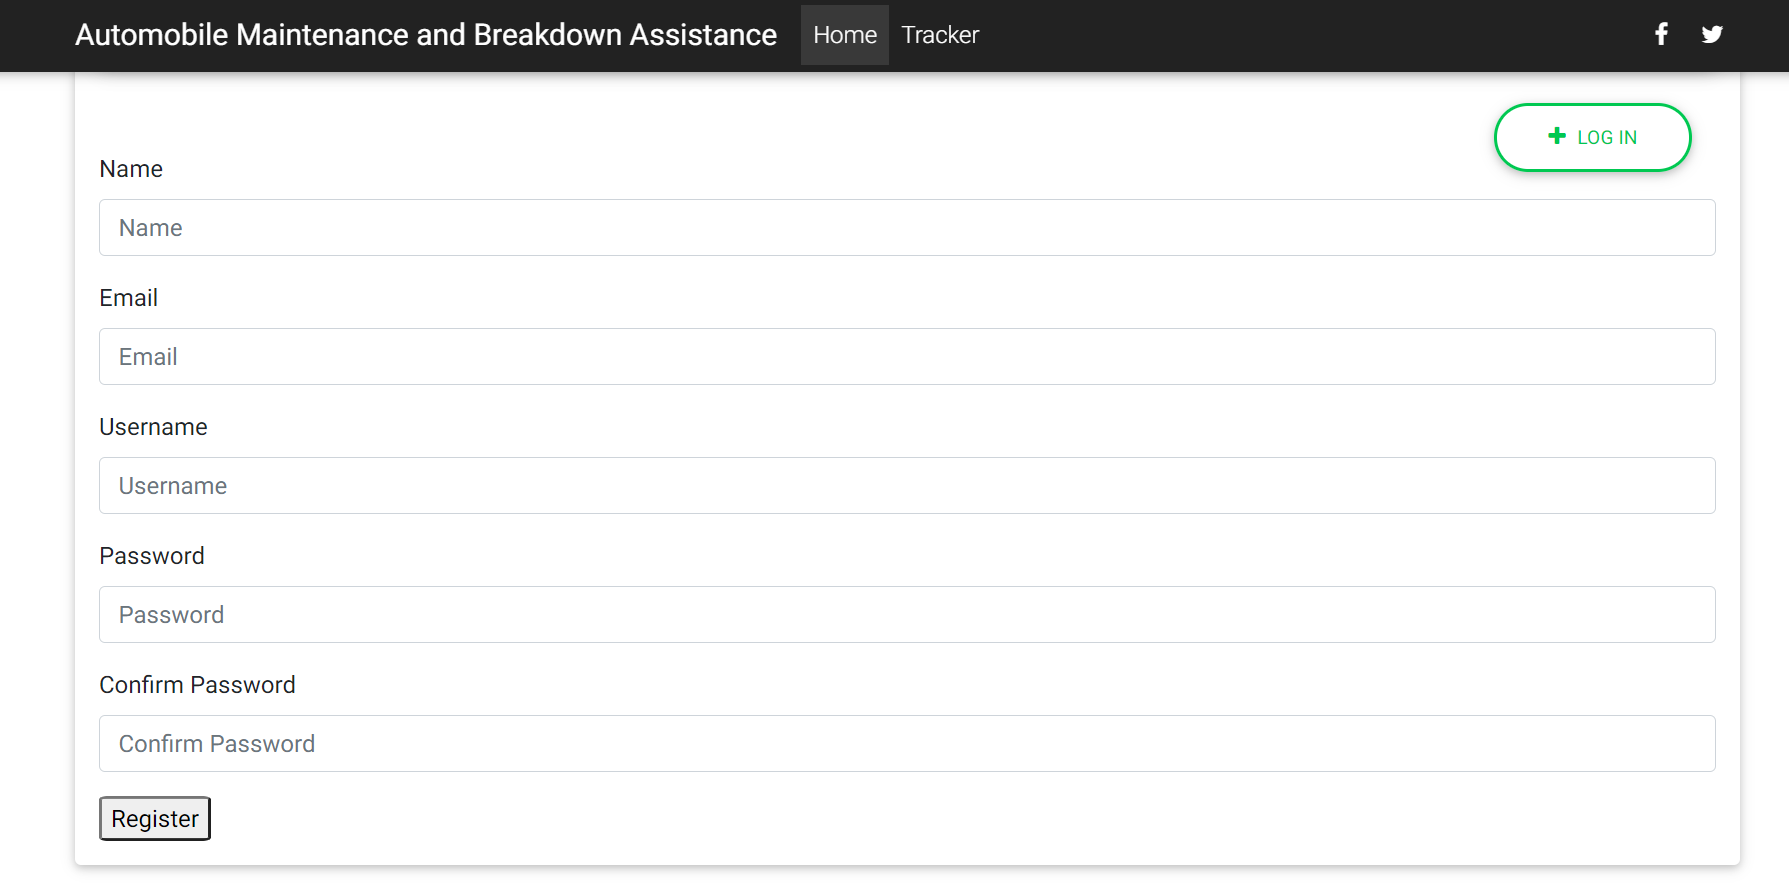
\includegraphics[width=15cm, height = 9cm]{register.PNG} \par 
        \caption{Register}
        \label{fig:register}
    \end{figure}
	
	\begin{figure}[!hbt]
		\centering
        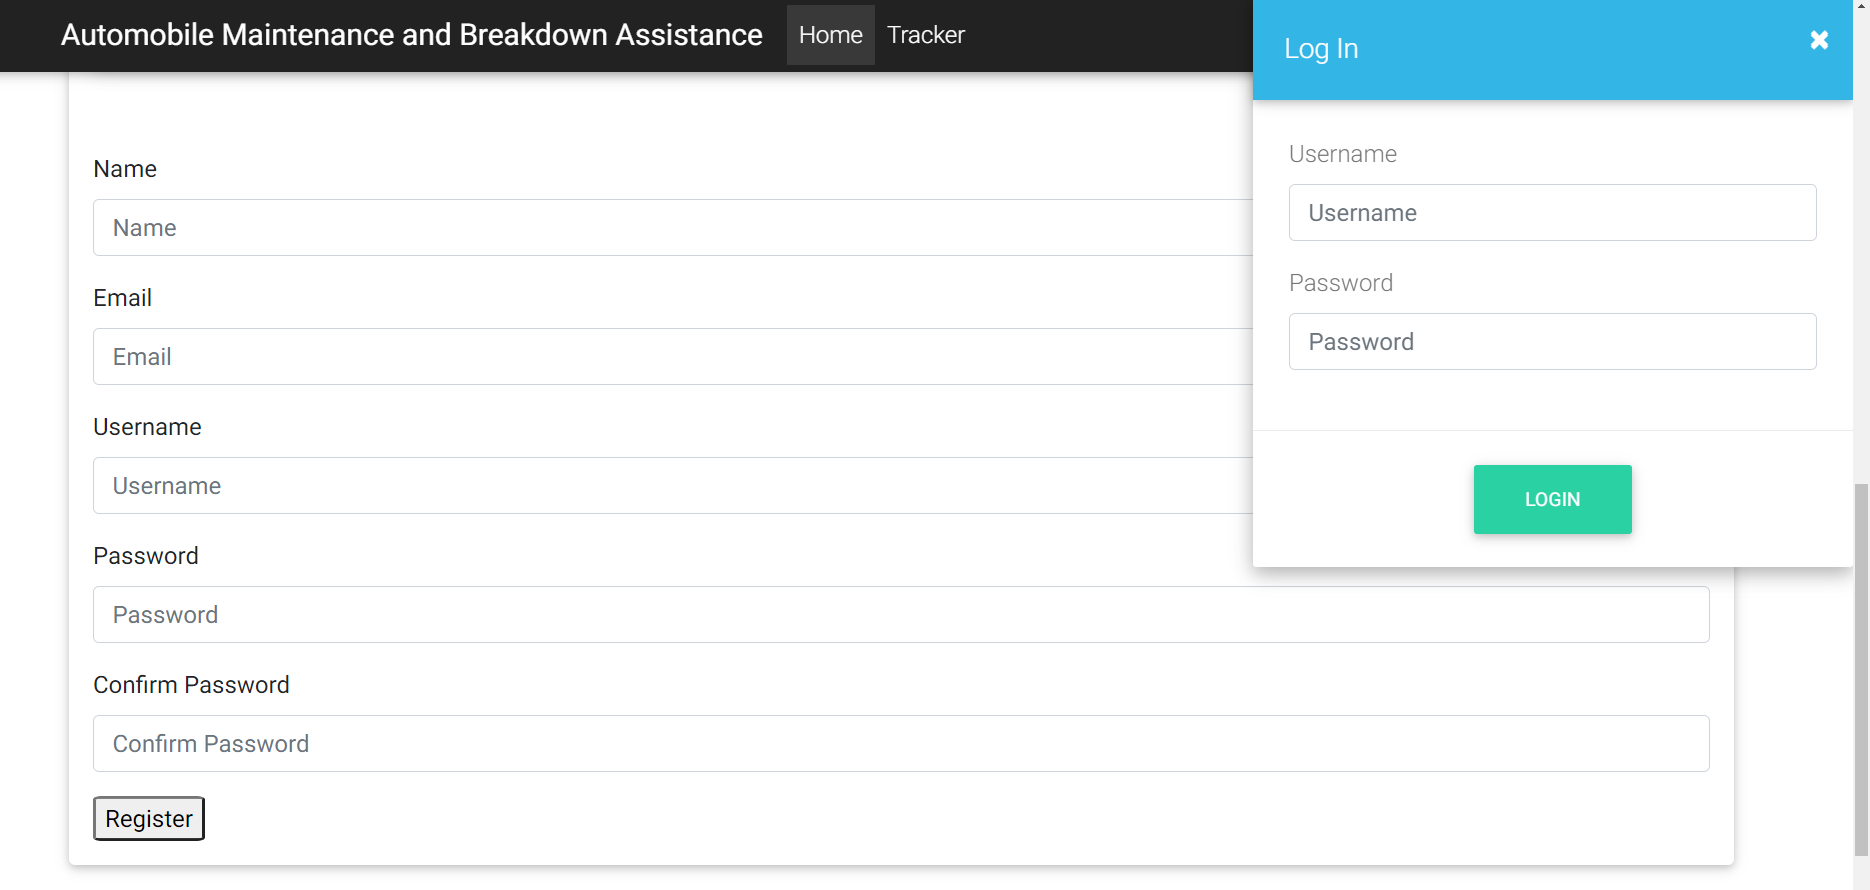
\includegraphics[width=15cm,height = 9cm]{login.PNG} \par 
        \caption{LogIn}
        \label{fig:login}
    \end{figure}
	
	\begin{figure}[!hbt]
		\centering
        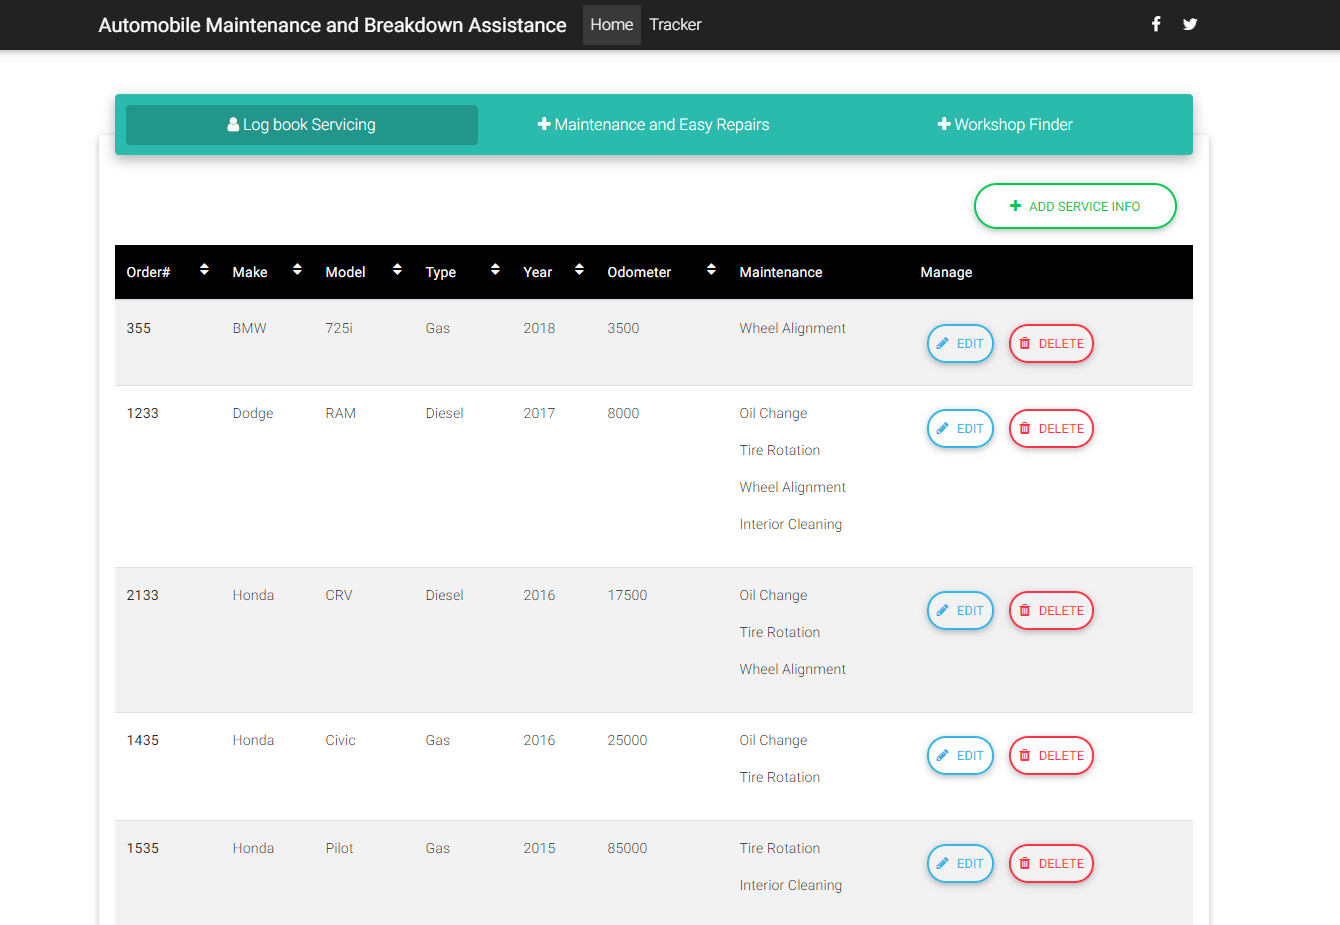
\includegraphics[width=\linewidth,height = 12cm]{m1.PNG} \par
        \caption{Log Book Servicing}
        \label{fig:LogBook}
    \end{figure}
    
    \begin{figure}[!hbt]
		\centering
        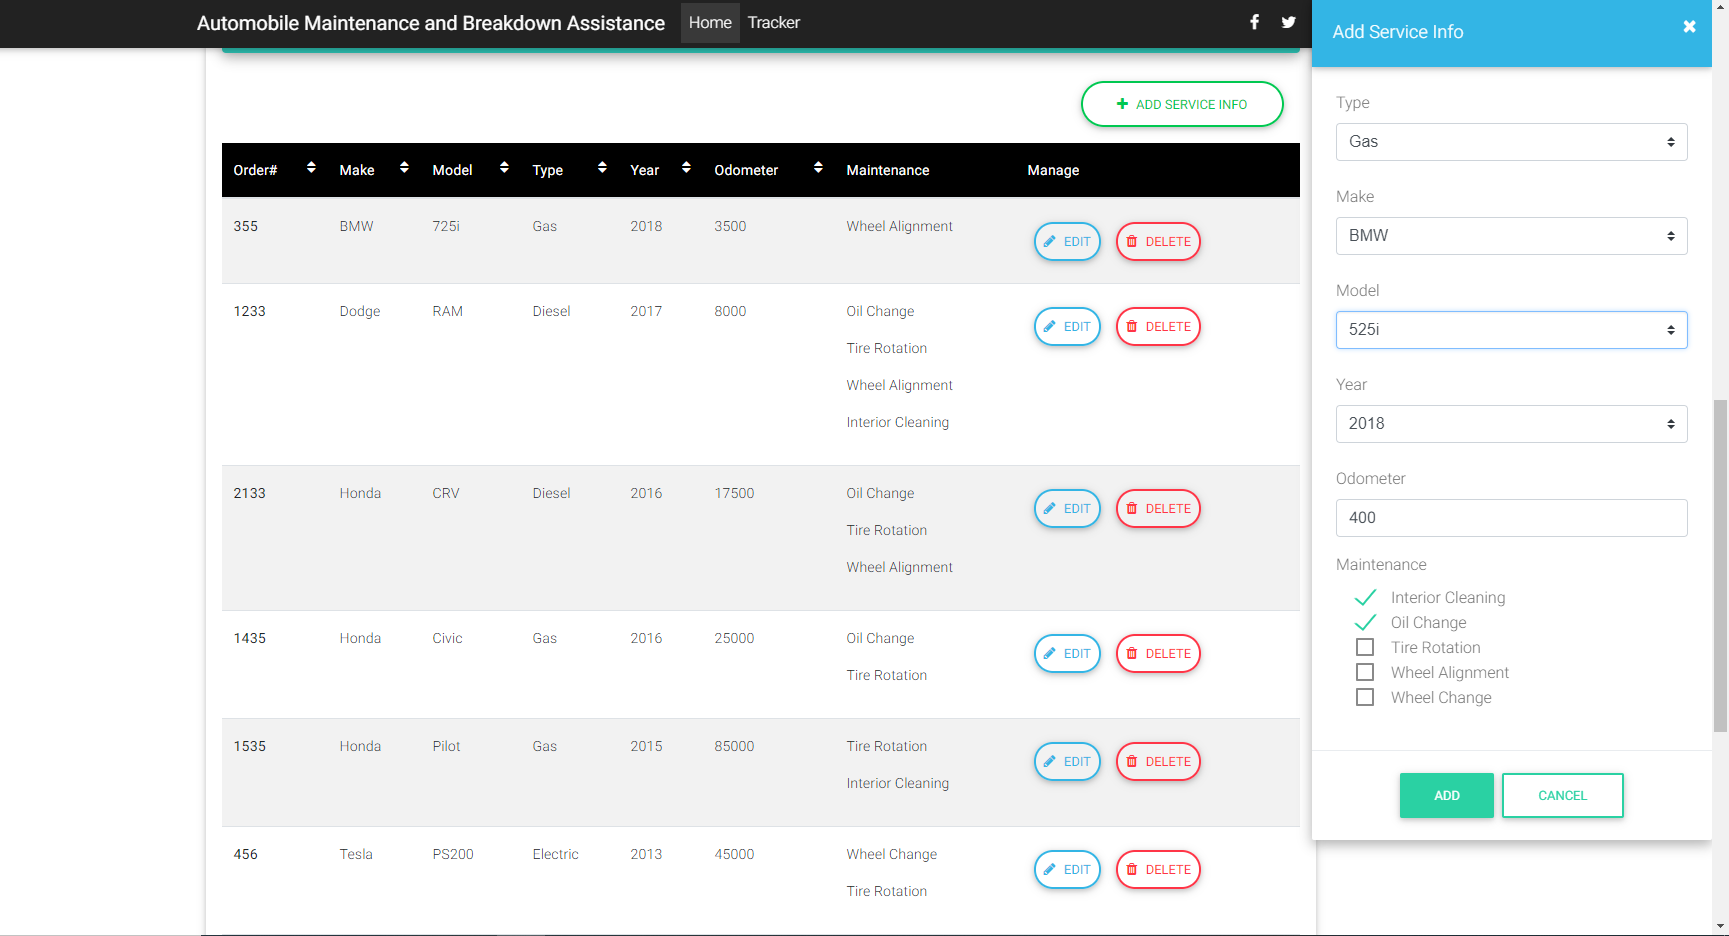
\includegraphics[width=\linewidth,height = 10cm]{m1.1.PNG} \par
        \caption{Add Service Info}
        \label{fig:Add Service}
    \end{figure}
    
    \begin{figure}[!hbt]
		\centering
        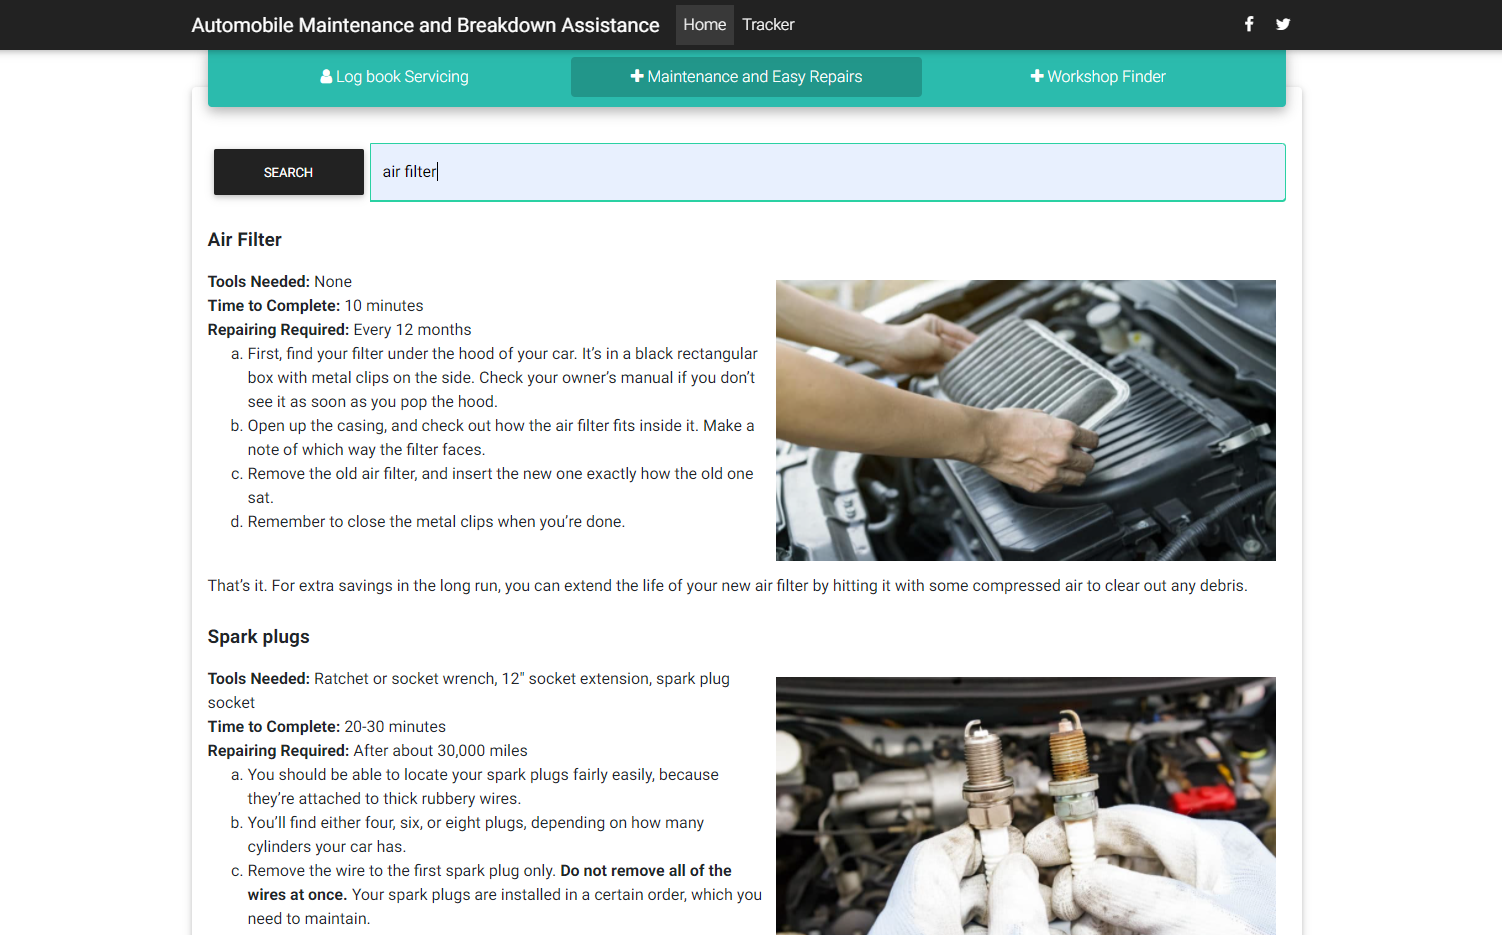
\includegraphics[width=\linewidth,height= 11cm]{m2.PNG} \par
        \caption{Search for Maintenance Info}
        \label{fig:Maintenance}
    \end{figure}
    
    \begin{figure}[!hbt]
		\centering
        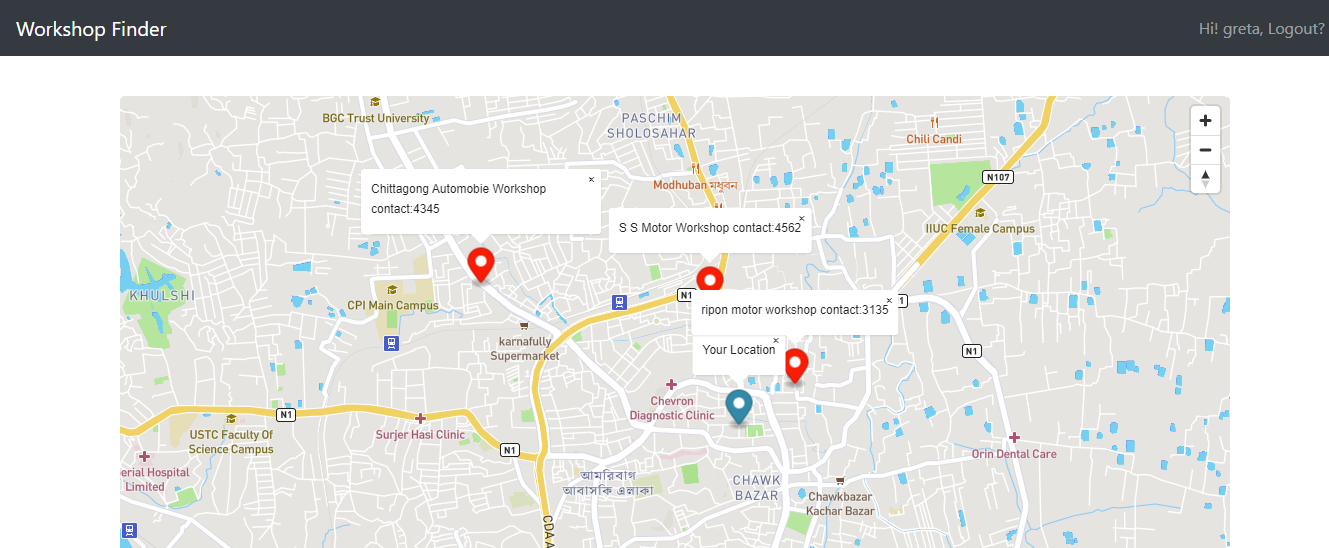
\includegraphics[width=\linewidth]{map.PNG} \par
        \caption{Locating nearest workshop}
        \label{fig:workshop}
    \end{figure}
    
    \begin{figure}[!hbt]
		\centering
        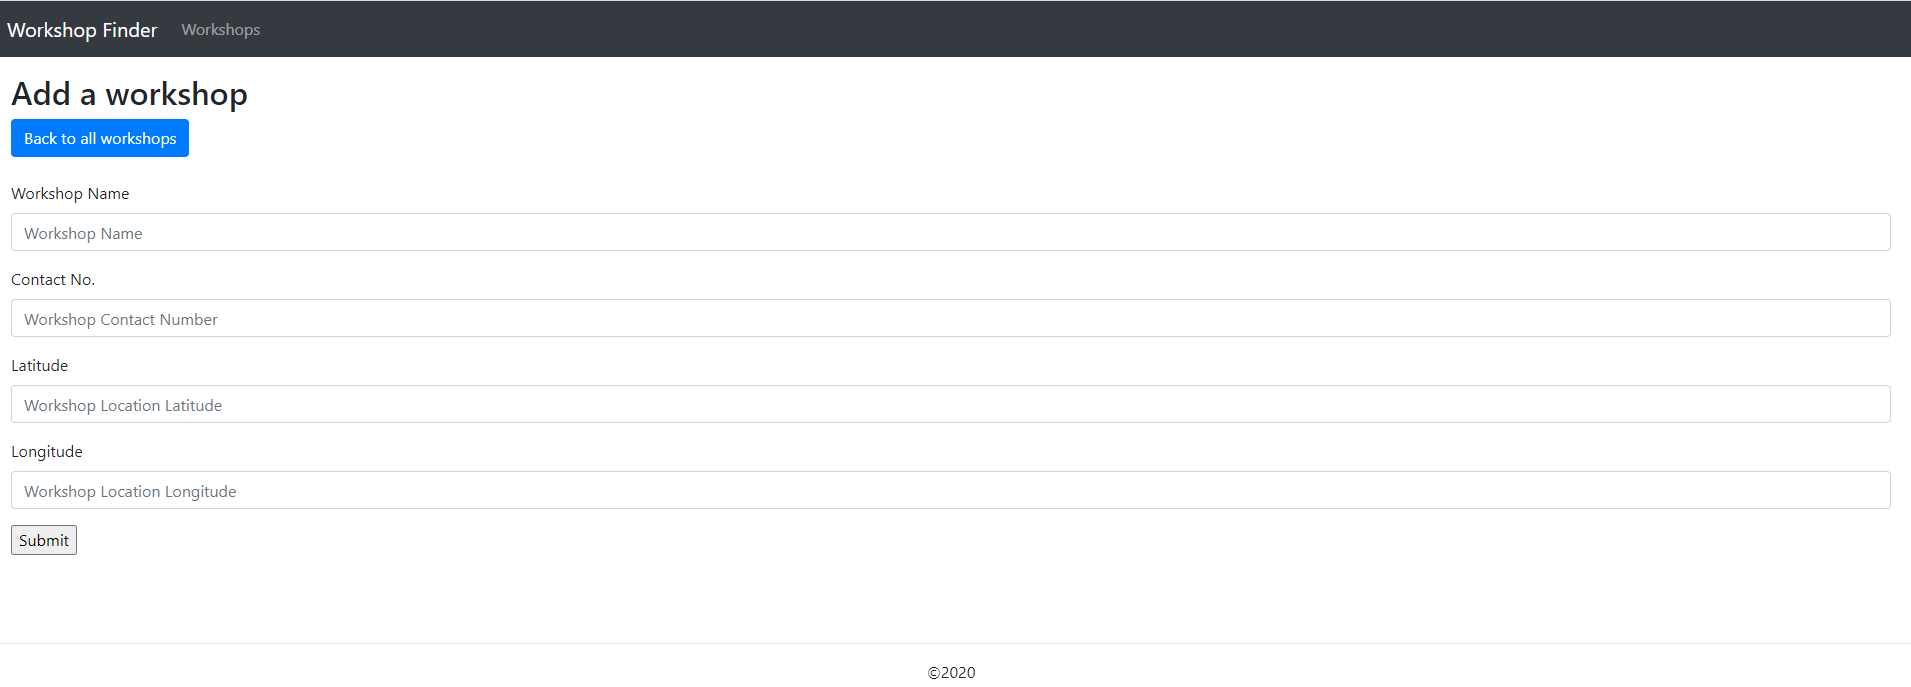
\includegraphics[width=\linewidth]{3.2.PNG} \par
        \caption{Adding workshop information by Admin}
        \label{fig:add workshop}
    \end{figure}
    
    \begin{figure}[!hbt]
		\centering
        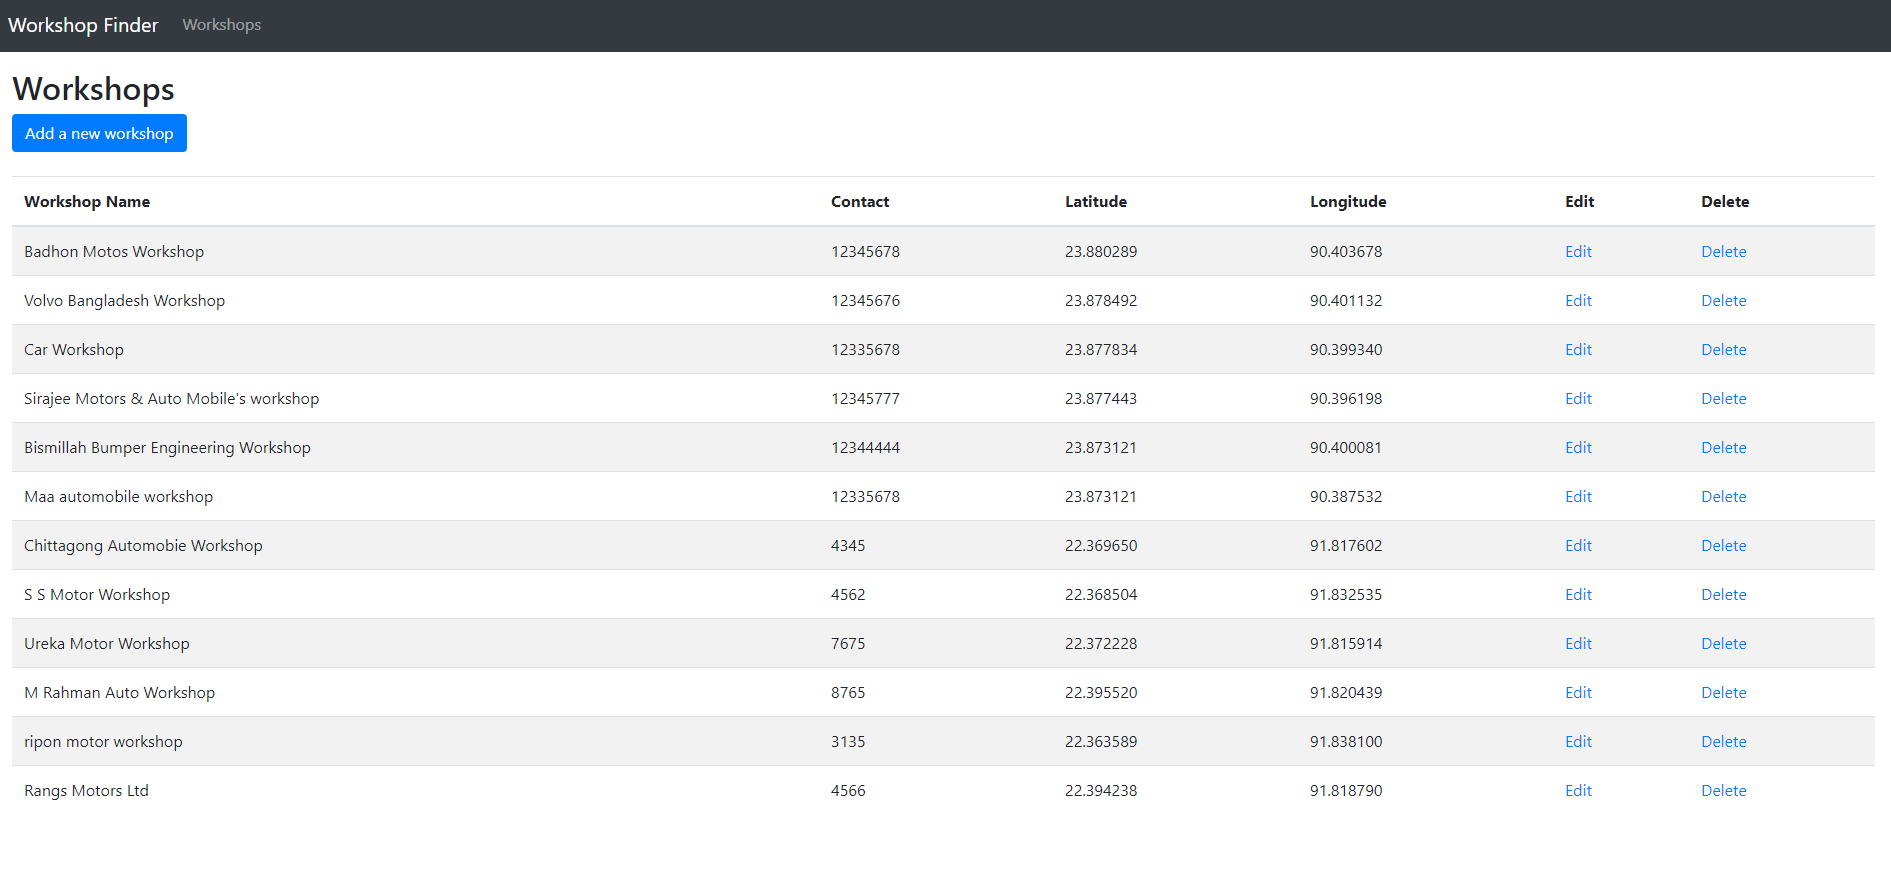
\includegraphics[width=\linewidth]{m3.1.PNG} \par
        \caption{Editing Workshop List}
        \label{fig:edit workshop}
    \end{figure}
    
    

\section{Testing and sustainability plan}
A software product has to be tested before deploying it in the market to determine errors that were made inadvertently during software design and construction. In order to avoid any sort of inconvenience, we consider different strategies and test our web application in the following sections.
	\subsection{Requirements/specifications-based system level test cases}
	Mocha is a feature-rich JavaScript test framework running on Node.js which has been employed to perform testing of our project by mapping exceptions to correct test cases. We also used Chai which is an assertion library. Unit testing of the project has been performed. For example, in our register function that registers new user to our service, we checked if the url is resolved, whether the users can see the registration form and whether they can actually sign up using this form. Mocha along with Chai assertion library includes all the functionalities required for this purpose. 
	\subsection{Traceability of test cases to use cases}
	The traceability of test cases to use case is represented below:\\
    \subsubsection{Authentication error}
    Using a wrong password will show authentication error that is showed in Figure\ref{fig:AE}.
	\begin{figure}[!hbt]
		\centering
        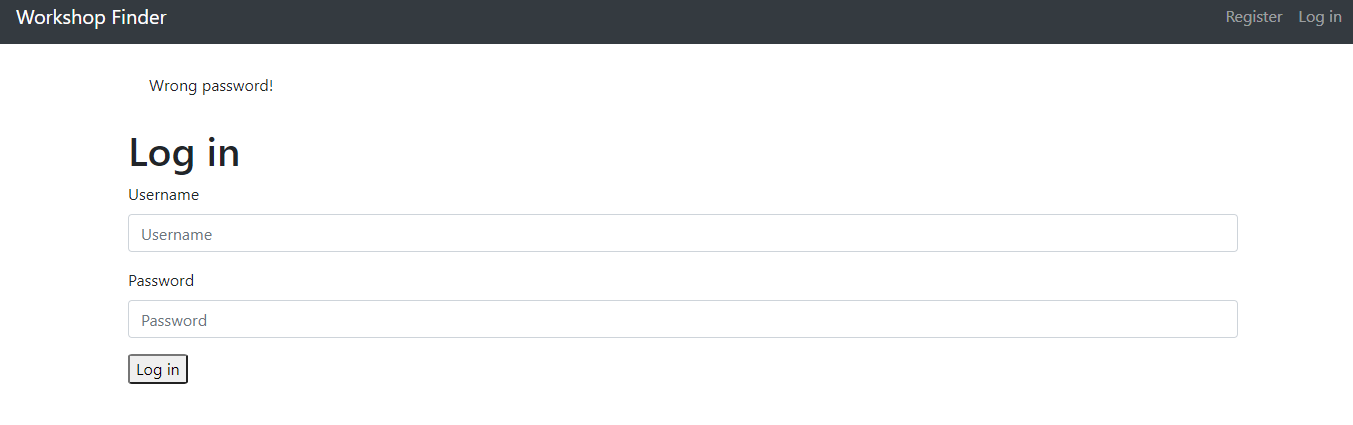
\includegraphics[width=\linewidth]{testcase wrong password.PNG} \par
        \caption{Authentication Error}
        \label{fig:AE}
    \end{figure}
    \newpage
    \subsubsection{View Workshop List only by Admin}
    Only admin can view workshop lists that is showed in Figure \ref{fig:ViewAdmin}.
    
	\begin{figure}[!hbt]
		\centering
        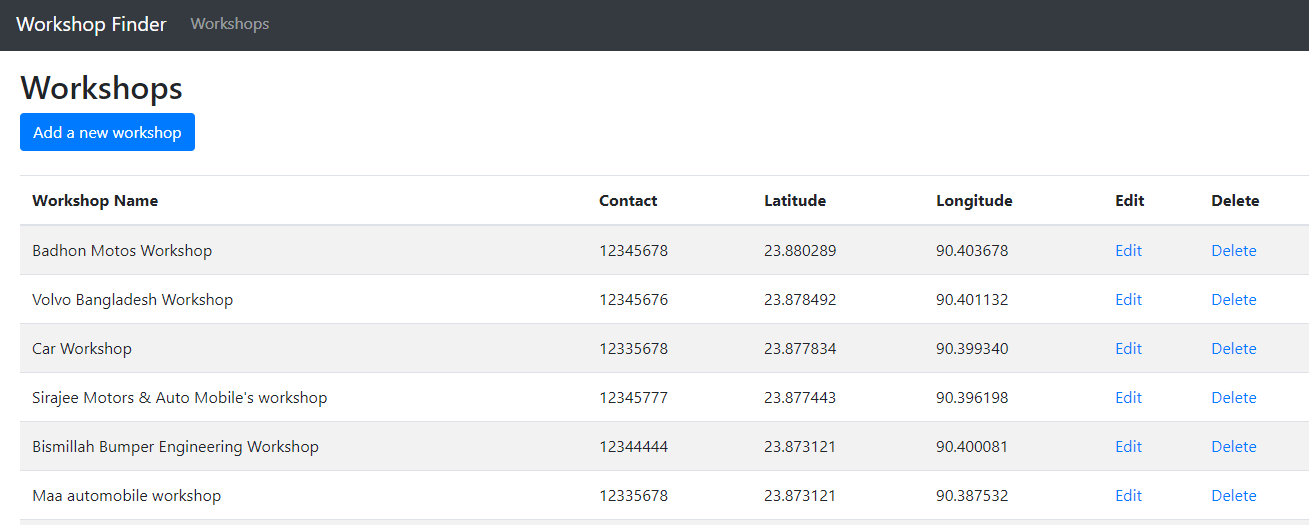
\includegraphics[width=\linewidth]{testcase2.PNG} \par
        \caption{View Workshop List only by Admin}
        \label{fig:ViewAdmin}
    \end{figure}
    
    \subsubsection{Add to service log option}
    
    Only authenticated user can add or edit to service log that is showed in Figure \ref{fig:AE}.
	\begin{figure}[!hbt]
		\centering
        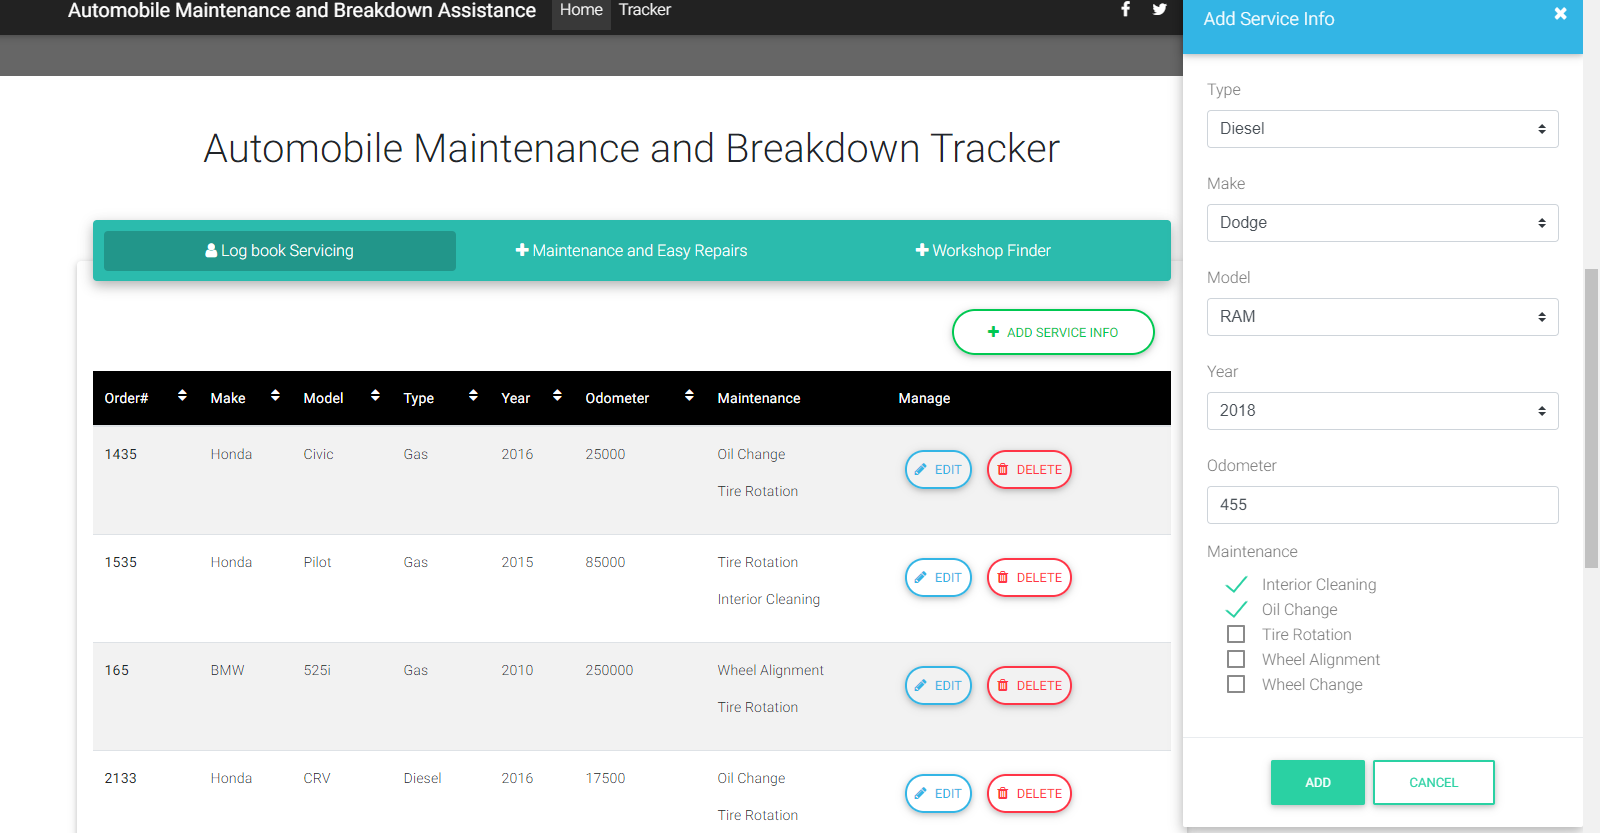
\includegraphics[width=\linewidth]{addproduct.PNG} \par
        \caption{Add to service log option}
        \label{fig:ViewAdmin}
    \end{figure}
    \newpage
    \subsubsection{Add a new Workshop only by Admin}
    
    Admin can add a new workshop that is showed in Figure \ref{fig:AddW}.
    \begin{figure}[!hbt]
		\centering
        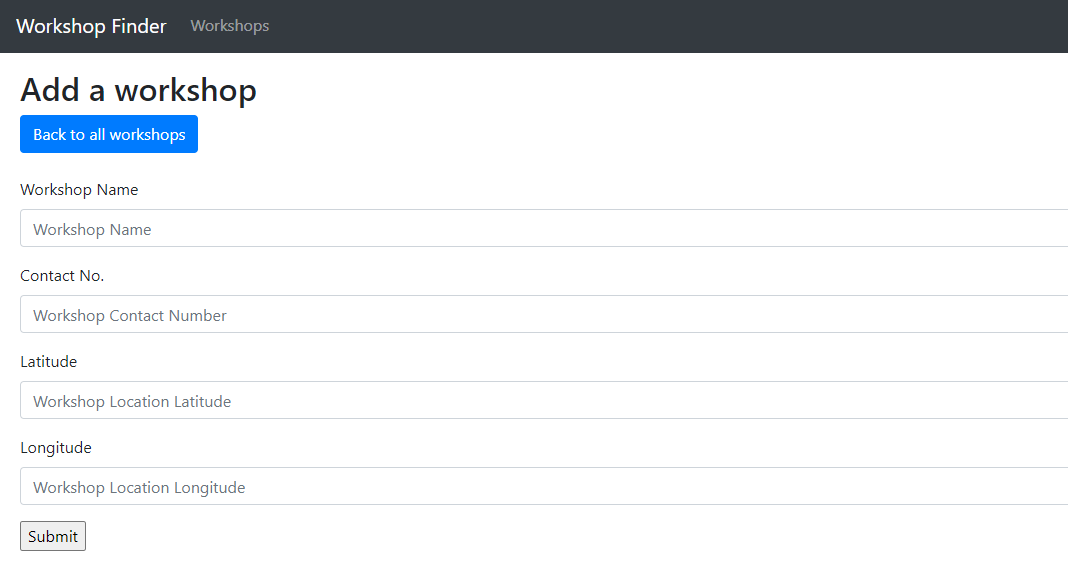
\includegraphics[width=\linewidth]{test add new workshop.PNG} \par
        \caption{Add a new Workshop only by Admin}
        \label{fig:AddW}
    \end{figure}
    
    \subsubsection{View Nearest Workshop Location}
    User can retrieve nearest 3 to 4 workshops around his/her present location that is showed in Figure \ref{fig:VL}.
    
	\begin{figure}[!hbt]
		\centering
        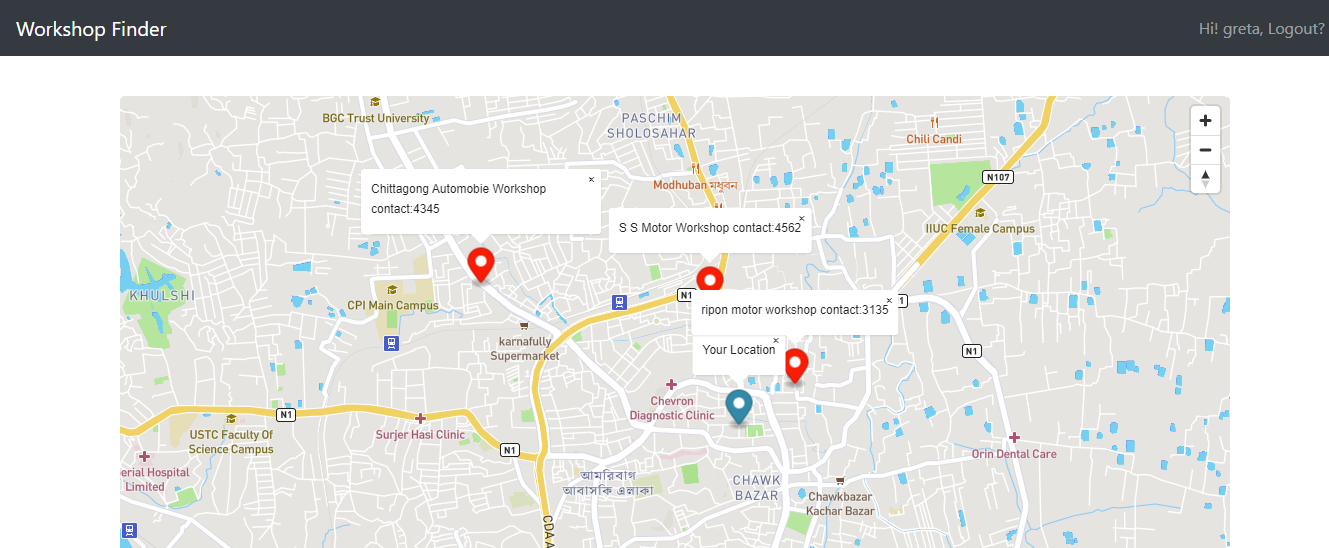
\includegraphics[width=\linewidth]{map.PNG} \par
        \caption{View Nearest Workshop Location}
        \label{fig:VL}
    \end{figure}
	\newpage
	\subsubsection{Verified user Authentication}
	A  user cannot register twice using same username or email id  that is showed in Figure \ref{fig:VUA}.
    \begin{figure}[!hbt]
		\centering
        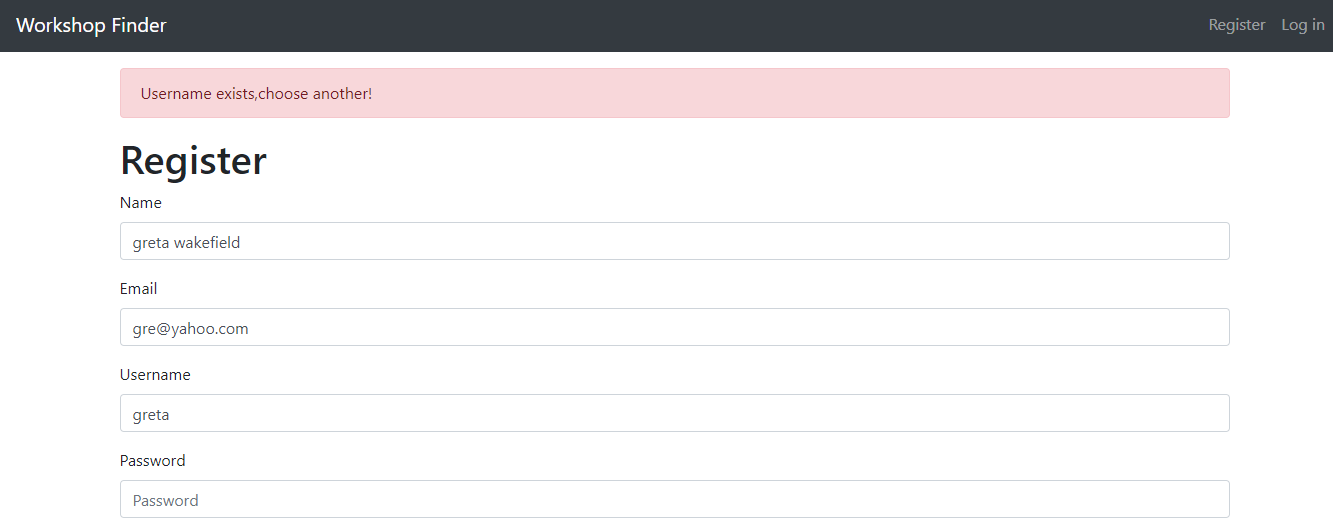
\includegraphics[width=\linewidth]{testcase registering twice.PNG} \par
        \caption{Verified user Authentication}
        \label{fig:VUA}
    \end{figure}
    
    
	\begin{table}[ht]
    \caption{Traceability of test cases}
    \label{tab:traceability}
    \begin{center}
    
    \begin{tabular}{|c|c|c|}
    \hline
    \textbf{Test Case ID} & \textbf{Description} & \textbf{Use Case Tested} 
    \\ \hline
    
    6.2.1
    & \begin{tabular}[c]{@{}c@{}}To examine if the user can enter without authentication.\end{tabular}
    & 6\\
    \hline
    	
  
    6.2.2  
    & \begin{tabular}[c]{@{}c@{}}To examine if the authenticated\\ admin can view the workshop list. \end{tabular} & 5\\
    \hline
    
    
    6.2.3
    & \begin{tabular}[c]{@{}c@{}}To examine if the authenticated user \\can add into service log. \end{tabular} 
     & 7 \\\hline
    
    6.2.4
    & \begin{tabular}[c]{@{}c@{}}To examine if the authenticated admin can add a new workshop. \end{tabular} 
    & 2\\ \hline
    
    6.2.5
    & \begin{tabular}[c]{@{}c@{}} To examine if the authenticated user\\ can find a nearest workshop location. \end{tabular}
    & 4 \\ \hline
    
    6.2.6
    & \begin{tabular}[c]{@{}c@{}} To examine if an already authenticated\\ user cannot register again. \end{tabular}
    & 6 \\ \hline
    
    
    \end{tabular}
    \end{center}
    \end{table}
    
	
	
	
	
	
	
	
	
	
	
	\subsection{Techniques used for test generation}
	A goal oriented approach was followed for generating test cases in order to check whether the entire project is functioning properly. Each functions were tackled one by one. Random test generation was not performed because the scope of our project was small and limited. Implementing such random approaches might risk the possibility of test cases to reach out of scope.
	\subsection{Assessment of the goodness of your test suite}
	According to the WebApp Project Metrics as defined by Pressman et al. in \cite{DUMMY:1} we perform an assessment of the goodness of our WebApp.\\
	\textbf{Number of static Web Pages:} We included 3 static webpages. This measure  provides an indication of the overall size of the application and the effort required to develop it.\\
	\textbf{Number of dynamic Web Pages:} The WebApp comprises of 4 dynamic web pages.\\
	\textbf{Number of internal page links:} This measure provides an indication of the degree of architectural coupling within the WebApp.\\
	\subsection{Sustainability Plan}
	To assess how our automobile maintenance and breakdown assistance service will meet the needs of current context without compromising the ability of future generations to meet their needs we undertake a sustainability plan which is discussed in the following subsections.
	\begin{subs}
		\subsubsection{Scalability}
	    Software scala
	    bility is an attribute of the software product to increase its capacity and functionalities based on its users' demand. We designed this web application using node.js server considering scalability since node.js has a built-in module,'cluster', which makes it convenient to implement cloning strategy on a single server. All types of automobile and workshop data were stored on Cloud Storage enabling data to be accessible from anywhere and available at any time.
		
		\subsubsection{Flexibility / Customization}
		The term flexibility in software engineering refers to the ease with which the system can adapt to external changes or new configurations. Node.js is a JavaScript based open source server environment. Our web application was designed using node.js which is a module-based technology. This technology enables in adding new features and expanding functionalities by simply creating new modules and performing export/import functions to integrate these updated features to the main server file which demonstrates its flexibility. Thus, our product can be customized and updated based on user's personal preferences and feedback. \\
	\end{subs}

\textbf{Acknowledgment}\\
The entire process of this software development beginning from planning to coding and testing required a lot of guidance and assistance from a number of people. It has been an enriching and fulfilling experience both professionally and personally.\\ Firstly, I would like to express my deep gratitude and honour to my course teachers Mir. Md. Saki Kowsar, Assistant Professor, Department of Computer Science & Engineering, Chittagong University of Engineering & Technology (CUET) for his guidance, encouragement and continuous support during our project work. I am thankful for his many critical questions, forcing me to see things from different perspectives, and his magnificent support throughout the entire time. \\I owe my gratitude to Ashim Dey, Lecturer, Department of Computer Science & Engineering, Chittagong University of Engineering & Technology (CUET) for guiding us and providing necessary information and suggestions. I am thankful for his constant encouragement, support, and guidance. \\I would also like to thank my team members Adrita Barua and Tarek Hossain for their wholehearted effort, constant hard work and dedication to make this project a successful one. \\Finally, I want to thank my father and mother for their unconditional love, support, encouragement, and contribution all throughout my life and academic career in every aspect along the years.\\

		
		
		
		
 \printindex % uncomment if causes any problem
% \lipsum[1-5]
% \layout
\bibliographystyle{splncs03_unsrt} 
\bibliography{bibliography}
\end{document}
